%提出するレポートの書式はこのtemplateファイルに沿って作成してください。
%特に表紙・概要の書式は変えないで下さい。

\documentclass[a4j]{jarticle}

\usepackage[dvipdfmx]{graphicx}
% \usepackage{epsbox}
\usepackage{url}
\usepackage{here}
\usepackage{ascmac}

\setlength{\headsep}{-5mm}
\setlength{\oddsidemargin}{0mm}
\setlength{\textwidth}{165mm}
\setlength{\textheight}{230mm}
\setlength{\footskip}{20mm}

\title{
\vspace{30mm}
{\bf 高知工科大学様}\\
\vspace{5mm}
大学掲示板(KUTBBS)\\
\vspace{5mm}
{\bf  内部設計書v1.0}
\vspace{90mm}
}
 \author{
\vspace{5mm}
グループ10 \\
\vspace{5mm}
Pathfinder \\
\vspace{5mm}
\vspace{10mm}
}

 \begin{document}
\maketitle
\newpage
\tableofcontents
\newpage


 \section{システム概要}
本システムは、学生が陥りやすいトラブルや、学生自身の学習における課題や悩みを自主的に解決するため の掲示板型のウェブアプリケーションである。 学生同士が問題をネット上でかつ匿名に解決できるようにするために開発するシステムが、本システムである。 利用する対象は、本校の学生である。また管理者は、本校の事務員を想定している。\\
 本システムは、メインシステムとして下記に示す「ユーザシステム」、「掲示板システム」、「管理者システム」 の 3 つを実装しており、各システムを構成するサブシステムも併せて以下に示す。
\begin{itemize}
\item 掲示板システム
	\begin{itemize}
	\item 掲示板サブシステム
	\item 検索サブシステム
	\item コレクトボタンサブシステム
	\item 通報サブシステム
	\item 通知サブシステム
	\end{itemize}
\item ユーザシステム
	\begin{itemize}
	\item アカウント登録サブシステム
	\item ログインサブシステム
	\item マイページサブシステム
	\item ブックマークサブシステム
	\item お知らせ表示サブシステム
	\end{itemize}
\item 管理者システム
	\begin{itemize}
	\item 管理者ログインサブシステム
	\item 子管理者管理サブシステム
	\item お知らせ編集サブシステム
	\item 掲示板編集サブシステム
	\item ユーザ管理サブシステム
	\end{itemize}
\end{itemize}
 \section{動作環境}
本システムの動作環境は以下の通りである。
\begin{itemize}
\item 動作環境
	\begin{itemize}
	\item CPU : ARM Cortex-A53 1GHz以上
	\item GPU : Broadcom VideoCore IV
	\item メモリ : 2GB以上
	\item ストレージ : 4GB eMMC / SDカードPIN
	\item OS
	\begin{itemize}
		\item Linux version 7
		\item ubuntu version 18.04
		\item MacOS
		\item Windowss7 , 8 , 10
		\item iOS 10.0
	\end{itemize}
	\item webサーバ : AWS EC2
	\item Appサーバ : Ruby on Rails version 5.1.4
	\item RDBMS : MySQL version 8.0
	\end{itemize}
\item 使用ブラウザ : GoogleChrome62.0 , Firefox version 57.0% , Safari11.0.1
\end{itemize}
\section{開発環境}
本システムの開発環境は以下の通りである。
\begin{itemize}
\item OS
	\begin{itemize}
		\item Linux version 7
		\item ubuntu version 18.04
		\item MacOS
		\item Windowss7 , 8 , 10
		\item iOS 10.0
	\end{itemize}
\item HTML : version5
\item 使用言語
	\begin{itemize}
	\item ruby version 2.4.2
	\item Ruby on Rails version 5.1.4
	\item CSS
	\item JavaScript
	\end{itemize}
\item サーバ :
\item データベース : MySQL version 8.0
\item webサーバ : AmazonWebServices
\end{itemize}
 \section{内部設計書作成方針}
\subsection{コーディング規約}
\subsubsection{命名規約}
\begin{itemize}
\item 変数名・メソッド名\\
‐ 小文字始まりとする\\
‐ 基本的に意味のある単語を使用する\\
‐
\end{itemize}
\begin{itemize}
\item 定数\\
‐ 全て大文字を使用する\\
\end{itemize}
\begin{itemize}
\item クラス名・構造体名\\
‐ 変数名・メソッド名を同様に意味のある単語を使用する\\
‐ 大文字始まりとする\\
‐ 複数の単語を組み合わせる際は先頭文字を大文字で表記する\\
\end{itemize}
\subsubsection{コーディングスタイル}
\begin{itemize}
\item インデント\\
‐ インデントにはタブを使用する(半角スペース4文字)
\end{itemize}
\begin{itemize}
\item 括弧\\
‐ 中括弧は改行して始める\\
‐ 小括弧の前後にはスペースを使用しない
\end{itemize}
\begin{itemize}
\item 演算子\\
‐ 演算子の前後には半角スペースを一文字使用する
\end{itemize}
\subsection{設計書作成環境}
内部設計書の作成環境は,表\ref{tab:creating_environment}に示します。
\begin{table}[htb]
\caption{内部設計書の作成環境環境}
\begin{center}
  \begin{tabular}{|c|c|} \hline
    組版処理システム & LATEX,dvpdfmx\\ \hline
   文字コード &  UTF-8\\ \hline
    改行コード & LF(0x0A)  \\ \hline
  \end{tabular}
\label{tab:creating_environment}
\end{center}
\end{table}
\subsection{サーバ環境}
本システムを利用するためにはAmazon Web Services(AWS) の EC2 インスタンスを用いて実現します.サーバ環境は表\ref{tab:server_environment}に示します。
\begin{table}[htb]
\caption{サーバ側の動作環境}
\begin{center}
  \begin{tabular}{|c|c|} \hline
    対応OS & Ruby on Rails \\ \hline
   vCPU & 1\\ \hline
    メモリ(GiB) & 1  \\ \hline
    ストレージ & 30GB \\ \hline
  \end{tabular}
\label{tab:server_environment}
\end{center}
\end{table}
\subsection{テーブル設計}
本小節ではデータベース構成するテーブルについて示す。また、各カラムについても詳細も示す。

\subsubsection{ユーザテーブル(user)}
ユーザテーブルではユーザに関する情報を管理する。このテーブルの詳細は表\ref{tab:user} に示す。
\begin{table}[h]

  \caption{ユーザテーブル}
  \begin{center}
    \footnotesize
    \begin{tabular}{|l|l|l|c|c|l|l|} \hline

      \multicolumn{1}{|c|}{論理名}&\multicolumn{1}{|c|}{物理名}&\multicolumn{1}{|c|}{データ型}&精度&NULL&\multicolumn{1}{|c|}{オプション}&\multicolumn{1}{|c|}{PK/FK:mode}\\\hline \hline
      学籍番号&student\verb|_|id&char&7&×&-&\multicolumn{1}{|l|}{PK} \\\hline
      ユーザID&user\verb|_|id&varchar&20&×&-&- \\ \hline
      パスワード&password&varchar&20&×&-&- \\ \hline
      ハンドルネーム&write\verb|_|name&varchar&15&×&-&- \\ \hline
      保有ポイント&now\verb|_|point&int&4&×&-&- \\ \hline
      取り消しフラグ&cancel\verb|_|flag&int&1&×&-&- \\ \hline
      赤色フラグ&color\verb|_|flag&int&1&×&-&- \\ \hline
      斜体フラグ&diagonal\verb|_|flag&int&1&×&-&- \\ \hline
      太文字フラグ&bold\verb|_|letters\verb|_|flag&int&1&×&-&- \\ \hline
      通知フラグ&report\verb|_|flag&int&1&×&-&- \\ \hline
      管理者フラグ&administrator\verb|_|flag&int&1&○&-&- \\ \hline
      初回ログインフラグ&first\verb|_|login\verb|_|flag&int&1&×&-&- \\ \hline
      ログイン日数&count\verb|_|login&int&4&×&-&-\\ \hline
    \end{tabular}
    \label{tab:user}
  \end{center}
\end{table}

\begin{itemize}
\item 学籍番号\\
  ユーザの学籍番号を示す値であり、自テーブルの主キーである。NULL値は含まない。値は固定7文字の半角英数字にて構成される。
\item ユーザID\\
  ユーザを識別するためのIDを示す値である。NULL値は含まない。値は20文字以下の半角英数字にて構成される。
\item パスワード\\
  ユーザを識別するためのパスワードを示す値である。NULL値は含まない。値は20文字以下の半角英数字にて構成される。
\item ハンドルネーム\\
      ユーザがレス書き込みを行う際に表示する名前を示す値である。NULL値は含まない。値は15文字以下の文字列にて構成される。


\item 保有ポイント\\
  ユーザがログインした日数とコレクトボタンを10回以上押されたことで獲得したポイントを示す値である。NULL値は含まない。4桁(0001から9999)の数値にて構成される。

\item 取り消しフラグ\\
  拡張機能の1つであり、取り消し線を付与することを示す値である。NULL値は含まない。値は1桁の0(OFF)、1(ON)の数値にて構成される。

\item 赤色フラグ\\
  拡張機能の1つであり、赤色を付与することを示す値である。NULL値は含まない。値は1桁の0(OFF)、1(ON)の数値にて構成される。\\
\item 斜体フラグ\\
  拡張機能の1つであり、斜体を付与することを示す値である。NULL値は含まない。値は1桁の0(OFF)、1(ON)の数値にて構成される。

\item 太文字フラグ\\
  拡張機能の1つであり、太文字を付与することを示す値である。NULL値は含まない。値は1桁の0(OFF)、1(ON)の数値にて構成される。
\item 通知フラグ\\
  通知設定の切り替えを示す値である。NULL値は含まない。値は1桁の0(OFF)、1(ON)の数値にて構成される。
\item 管理者フラグ\\
  親管理者と子管理者を識別することを示す値である。値は1桁の0(子管理者)、1(親管理者)の数値にて構成される。\\
\item 初回ログインフラグ\\
  初回ログインを識別することを示す値である。NULL値は含まない。値は1桁の0(OFF)、1(ON)の数値にて構成される。

\item ログイン日数\\
  ユーザがログインをした日数を記録することを示す値である。NULL値は含まない。値は4桁(0001から9999)の数値にて構築される。

   \end{itemize}
\newpage
  \subsubsection{スレッドテーブル(thread)}
  スレッドテーブルではスレッドに関する情報を管理する。このテーブルの詳細は表\ref{tab:thread} に示す。
  \begin{table}[h]
    \caption{スレッドテーブル}
    \begin{center}
      %\fontsize{6.5pt}{30pt}\selectfont
      \footnotesize
      \begin{tabular}{|l|l|l|c|c|l|l|} \hline
        \multicolumn{1}{|c|}{論理名}&\multicolumn{1}{|c|}{物理名}&\multicolumn{1}{|c|}{データ型}&精度&NULL&\multicolumn{1}{|c|}{オプション}&\multicolumn{1}{|c|}{PK/FK:mode}\\\hline \hline
        スレッドID&thread\verb|_|id&int&5&×&\begin{tabular}{l}unsigned zerofill\\auto\verb|_|increment\end{tabular}&\multicolumn{1}{|l|}{PK} \\\hline
          スレッドカテゴリID&thread\verb|_|category\verb|_|id&int&3&×&\begin{tabular}{l}unsigned zerofill\\auto\verb|_|increment\end{tabular}&FK:thread\verb|_|category \\ \hline
            学籍番号&student\verb|_|id&char&7&×&-&\multicolumn{1}{|l|}{FK:user} \\\hline
            スレッドタイトル名&thread\verb|_|category\verb|_|name&varchar&50&×&-&- \\ \hline
            スレッド非表示フラグ&thread\verb|_|hide\verb|_|flag&int&1&×&-&- \\ \hline
            作成日時&created\verb|_|at&timestamp&-&×&default current\verb|_|timestamp&- \\ \hline
            更新日時&updated\verb|_|at&timestamp&-&×&\begin{tabular}{l}default current\verb|_|timestamp on \\update current\verb|_|timestamp\end{tabular}&- \\ \hline
      \end{tabular}

      \label{tab:thread}
    \end{center}
  \end{table}
  \begin{itemize}
  \item スレッドID\\
    自テーブルの主キーである。NULL値は含まない。値は5桁(00001から99999)の数値にて構成され自動追加される。\\

  \item スレッドカテゴリID\\
    スレッドカテゴリテーブルを参照する際の外部キーである。NULL値は含まない。値は3桁(001から999)の数値にて構成され自動追加される。\\

  \item 学籍番号\\
    ユーザテーブルを参照する際の外部キーである。NULL値は含まない。固定7文字の半角英数字にて構成される。\\

  \item スレッドタイトル名\\
    スレッドタイトルを示す値である。NULL値は含まない。値は50文字以下の文字列にて構成される。\\
  \item スレッド非表示フラグ\\
    管理者の操作権限でスレッドを非表示を示す値である。NULL値は含まない。値は1桁の数値で0(OFF)、1(ON)の数値にて構成される。\\
    例としてスレッド非表示フラグを1にした場合、ユーザ側からはスレッドが非表示になる。
  \item 作成日時\\
    レコードを作成した日付・時刻を示す値である。NULL値は含まない。レコードが作成されるたびに自動追加を行う。
  \item 更新日時\\
    レコードを更新した日付・時刻を示す値である。NULL値は含まない。レコードが更新されるたびに自動更新を行う。
  \end{itemize}
  \subsubsection{レステーブル(res)}
  レステーブルではレスに関する情報を管理する。このテーブルの詳細は表\ref{tab:ress} に示す。
  \begin{table}[h]
    \caption{レステーブル}
    \begin{center}
      %\fontsize{6.5pt}{30pt}\selectfont
      \footnotesize
      \begin{tabular}{|l|l|l|c|c|l|l|} \hline
        \multicolumn{1}{|c|}{論理名}&\multicolumn{1}{|c|}{物理名}&\multicolumn{1}{|c|}{データ型}&精度&NULL&\multicolumn{1}{|c|}{オプション}&\multicolumn{1}{|c|}{PK/FK:mode}\\\hline \hline
        レスID&res\verb|_|id&int&4&×&\begin{tabular}{l}unsigned zerofill\\auto\verb|_|increment\end{tabular}&PK \\\hline
          スレッドID&thread\verb|_|id&int&5&×&\begin{tabular}{l}unsigned zerofill\\auto\verb|_|increment\end{tabular}&\begin{tabular}{l}PK(res複合)\\FK:thread\end{tabular}\\\hline
              学籍番号&student\verb|_|id&char&7&×&-&\multicolumn{1}{|l|}{FK:user} \\\hline
              書き込みID&write\verb|_|id&char&8&×&-&-\\ \hline
              書き込み内容&write\verb|_|content&varchar&200&×&-&- \\ \hline
              コレクトプッシュ数&collect\verb|_|push\verb|_|count&int&4&×&-&- \\ \hline
              レス非表示フラグ&res\verb|_|hide\verb|_|flag&int&1&×&-&- \\ \hline
              作成日時&created\verb|_|at&timestamp&-&×&default current\verb|_|timestamp&- \\ \hline
      \end{tabular}

      \label{tab:ress}
    \end{center}
  \end{table}

  \begin{itemize}
  \item レスID\\
    自テーブルの主キーである。NULL値は含まない。値は4桁(0001から9999)の数値にて構成され自動追加される。
  \item スレッドID\\
    スレッドテーブルを参照する際の外部キーであり、スレIDとの複合主キーである。NULL値は含まない。値は5桁(00001から99999)の数値にて構成され自動追加される。
  \item 学籍番号\\
    ユーザテーブルを参照する際の外部キーである。NULL値は含まない。固定7文字の半角英数字にて構成される。\\
  \item 書き込みID\\
    ユーザが書き込みを行う際に表示するIDを示す値である。NULL値は含まない。値は固定8文字の半角英数字にて構成される。\\
  \item 書き込み内容\\
    書き込み内容を示す値である。NULL値は含まない。値は200文字以下の文字列にて構成される。\\
  \item コレクトボタンプッシュ数\\
    レスに対してコレクトボタンが押された回数を示す値である。NULL値は含まない。値は4桁(0001から9999)の数値にて構成される。\\
  \item レス非表示フラグ\\
    管理者の操作権限でレスを非表示を示す値である。NULL値は含まない。値は1桁の数値で0(OFF)、1(ON)の数値にて構成される。\\
    例としてレス非表示フラグを1にした場合、ユーザ側からはレスが非表示になる。

  \item 作成日時\\
    レコードを作成した日付・時刻を示す値である。NULL値は含まない。レコードが作成されるたびに自動追加される。
  \end{itemize}

  \subsubsection{スレッドカテゴリテーブル(thread\_category)}
  スレッドカテゴリテーブルは各カテゴリごとに分けられたスレッドの情報を管理する。このテーブルの詳細は表\ref{tab:thread_category} に示す。
  \begin{table}[h]
    \caption{スレッドカテゴリテーブル}
    \begin{center}
      %\fontsize{6.5pt}{30pt}\selectfont
      \footnotesize
      \begin{tabular}{|l|l|l|c|c|l|l|} \hline
        \multicolumn{1}{|c|}{論理名}&\multicolumn{1}{|c|}{物理名}&\multicolumn{1}{|c|}{データ型}&精度&NULL&\multicolumn{1}{|c|}{オプション}&\multicolumn{1}{|c|}{PK/FK:mode}\\\hline \hline
        カテゴリID&category\verb|_|no&int&3&×&\begin{tabular}{l}unsigned zerofill\\auto\verb|_|increment\end{tabular}&PK\\ \hline
          カテゴリ名&category\verb|_|name&varchar&15&×&-&-\\\hline
      \end{tabular}
      \label{tab:thread_category}
    \end{center}
  \end{table}

  \begin{itemize}
  \item カテゴリID\\
    自テーブルの主キーである。NULL値は含まない。値は3桁(001から999)の数値にて構築され自動追加される。
  \item カテゴリ名\\
    カテゴリの名前を示す値である。NULL値は含まない。値は15文字以下の文字列にて構成される。\\

  \end{itemize}

  \subsubsection{お気に入り掲示板テーブル(favorite\_bbs)}
  お気入り掲示板テーブルではブックマークとして登録したスレッド情報を管理する。このテーブルの詳細は表\ref{tab:favorite_bbs} に示す。
  \begin{table}[h]
    \caption{お気に入り掲示板テーブル}
    \begin{center}
      %\fontsize{6.5pt}{30pt}\selectfont
      \footnotesize
      \begin{tabular}{|l|l|l|c|c|l|l|} \hline
        \multicolumn{1}{|c|}{論理名}&\multicolumn{1}{|c|}{物理名}&\multicolumn{1}{|c|}{データ型}&精度&NULL&\multicolumn{1}{|c|}{オプション}&\multicolumn{1}{|c|}{PK/FK:mode}\\\hline \hline
        学籍番号&student\verb|_|id&char&7&×&-&\multicolumn{1}{|l|}{FK:user} \\\hline
        スレッドID&thread\verb|_|id&int&5&×&\begin{tabular}{l}unsigned zerofill\\auto\verb|_|increment\end{tabular}&FK:thread\\\hline
      \end{tabular}
      \label{tab:favorite_bbs}
    \end{center}
  \end{table}

  \begin{itemize}
  \item 学籍番号\\
    ユーザテーブルを参照する際の外部キーである。NULL値は含まない。固定7文字の半角英数字にて構成される。\\
  \item スレッドID\\
    スレッドテーブルを参照する際の外部キーである。NULL値は含まない。値は5桁(00001から99999)の数値にて構築され自動追加される。
  \end{itemize}



  \subsubsection{コレクトユーザテーブル(collect\_user)}
  コレクトユーザテーブルではコレクトボタンを押されたことに関する情報を管理する。このテーブルの詳細は表 \ref{tab:collect_user} に示す。
  \begin{table}[h]
    \caption{コレクトユーザテーブル}
    \begin{center}
      %\fontsize{6.5pt}{30pt}\selectfont
      \footnotesize
      \begin{tabular}{|l|l|l|c|c|l|l|} \hline
        \multicolumn{1}{|c|}{論理名}&\multicolumn{1}{|c|}{物理名}&\multicolumn{1}{|c|}{データ型}&精度&NULL&\multicolumn{1}{|c|}{オプション}&\multicolumn{1}{|c|}{PK/FK:mode}\\\hline \hline
        学籍番号&student\verb|_|id&char&7&×&-&\multicolumn{1}{|l|}{FK:user} \\\hline
        スレッドID&thread\verb|_|id&int&5&×&\begin{tabular}{l}unsigned zerofill\\auto\verb|_|increment\end{tabular}&FK:thread\\\hline
          レスID&res\verb|_|no&int&4&×&\begin{tabular}{l}unsigned zerofill\\auto\verb|_|increment\end{tabular}&FK:res \\\hline
      \end{tabular}
      \label{tab:collect_user}
    \end{center}
  \end{table}

  \begin{itemize}
  \item 学籍番号\\
    ユーザテーブルを参照する際の外部キーである。NULL値は含まない。固定7文字の半角英数字にて構成される。\\
  \item スレッドID\\
    スレッドテーブルを参照する際の外部キーである。NULL値は含まない。値は5桁(00001から99999)の数値にて構成され自動追加される。
  \item レスID\\
    レステーブルを参照する際の外部キーである。NULL値は含まない。値は4桁(0001から9999)の数値にて構成され自動追加される。
  \end{itemize}

  \subsubsection{不適切な単語登録テーブル(inadequacy\_word)}
  不適切な単語登録テーブルでは管理者が誹謗中傷や公序良俗に違反していると考えられる単語を登録した情報を管理する。このテーブルの詳細は表 \ref{tab:inadequacy_word} に示す。
  \begin{table}[h]
    \caption{不適切な単語登録テーブル}
    \begin{center}
      %\fontsize{6.5pt}{30pt}\selectfont
      \footnotesize
      \begin{tabular}{|l|l|l|c|c|l|l|} \hline
        \multicolumn{1}{|c|}{論理名}&\multicolumn{1}{|c|}{物理名}&\multicolumn{1}{|c|}{データ型}&精度&NULL&\multicolumn{1}{|c|}{オプション}&\multicolumn{1}{|c|}{PK/FK:mode}\\\hline \hline
        単語ID&word\verb|_|id&int&5&×&\begin{tabular}{l}unsigned zerofill\\auto\verb|_|increment\end{tabular}&PK\\\hline
          単語名&word\verb|_|name&varchar&200&×&-&- \\\hline
      \end{tabular}
      \label{tab:inadequacy_word}
    \end{center}
  \end{table}

  \begin{itemize}
  \item 単語ID\\
    自テーブルの主キーである。NULL値は含まない。値は5桁(00001から99999)の数値にて構成され自動追加される。
  \item 単語名\\
    管理者の操作権限で登録した単語を示す値である。NULL値は含まない。値は200文字以下の文字列にて構成される。
  \end{itemize}


  \subsubsection{通報テーブル(report)}
  通報テーブルではユーザが誹謗中傷や公序良俗に違反するなどの不適切な内容であると判断したスレッドまたはレスを管理者に通報した時の情報を管理する。また、通報した内容の情報も管理する。このテーブルの詳細は表 \ref{tab:report} に示す。
  \begin{table}[h]
    \caption{通報テーブル}
    \begin{center}
      %\fontsize{6.5pt}{30pt}\selectfont
      \footnotesize
      \begin{tabular}{|l|l|l|c|c|l|l|} \hline
        \multicolumn{1}{|c|}{論理名}&\multicolumn{1}{|c|}{物理名}&\multicolumn{1}{|c|}{データ型}&精度&NULL&\multicolumn{1}{|c|}{オプション}&\multicolumn{1}{|c|}{PK/FK:mode}\\\hline \hline
        通報ID&report\verb|_|id&int&5&×&\begin{tabular}{l}unsigned zerofill\\auto\verb|_|increment\end{tabular}&PK\\\hline
          通報ユーザID&report\verb|_|user\verb|_|id&varchar&20&×&-&FK:user \\ \hline
          スレッドID&thread\verb|_|id&int&5&×&\begin{tabular}{l}unsigned zerofill\\auto\verb|_|increment\end{tabular}&FK:thread\\\hline
            レスID&res\verb|_|id&int&4&×&\begin{tabular}{l}unsigned zerofill\\auto\verb|_|increment\end{tabular}&FK:res \\\hline
              通報内容&report\verb|_|content&varchar&200&×&-&-\\ \hline
              通報日時&report\verb|_|at&timestamp&-&×&default current\verb|_|timestamp&- \\ \hline
      \end{tabular}
      \label{tab:report}
    \end{center}
  \end{table}

  \begin{itemize}
  \item 通報ID\\
    自テーブルの主キーである。NULL値は含まない。値は5桁(00001から99999)の数値にて構成され自動追加される。
  \item 通報ユーザID\\
    ユーザテーブルを参照する際の外部キーである。NULL値は含まない。値は20文字以下の半角英数字にて構成される。\\

  \item スレッドID\\
    スレッドテーブルを参照する際の外部キーである。NULL値は含まない。値は5桁(00001から99999)の数値にて構成され自動追加される。
  \item レスID\\
    レステーブルを参照する際の外部キーである。NULL値は含まない。値は4桁(0001から9999)の数値にて構成され自動追加される。
  \item 通報内容\\
    通報内容を示す値である。NULL値は含まない。値は200文字以下の文字列にて構成される。\\

  \item 通報日時\\
    レコードを作成した日付・時刻を示す値である。NULL値は含まない。レコードが作成されるたびに自動追加を行う。
  \end{itemize}

  \subsubsection{凍結ユーザテーブル(suspend)}
  凍結ユーザテーブルでは迷惑行為が改善されないユーザのアカウントを凍結した情報を管理する。このテーブルの詳細は表 \ref{tab:suspend} に示す。

  \begin{table}[h]
    \caption{凍結ユーザテーブル}
    \begin{center}
      \fontsize{6.5pt}{30pt}\selectfont
      \footnotesize
      \begin{tabular}{|l|l|l|c|c|l|l|} \hline
        \multicolumn{1}{|c|}{論理名}&\multicolumn{1}{|c|}{物理名}&\multicolumn{1}{|c|}{データ型}&精度&NULL&\multicolumn{1}{|c|}{オプション}&\multicolumn{1}{|c|}{PK/FK:mode}\\\hline \hline
        凍結ID&suspend\verb|_|id&int&4&×&\begin{tabular}{l}unsigned zerofill\\auto\verb|_|increment\end{tabular}&PK\\\hline
          学籍番号&student\verb|_|id&char&7&×&-&\multicolumn{1}{|l|}{FK:user} \\\hline
      \end{tabular}
      \label{tab:suspend}
    \end{center}
  \end{table}

  \begin{itemize}
  \item 凍結ID\\
    自テーブルの主キーである。NULL値は含まない。値は4桁(0001から9999)の数値にて構成され自動追加される。
  \item 学籍番号\\
    ユーザテーブルを参照する際の外部キーである。。NULL値は含まない。値は固定7文字の半角英数字にて構成される。\\
  \end{itemize}

  \subsubsection{お知らせテーブル(news)}
  お知らせテーブルではお知らせに関する情報を管理する。このテーブルの詳細は表 \ref{tab:news} に示す。
  \begin{table}[h]
    \caption{お知らせテーブル}
    \begin{center}
      \fontsize{6.5pt}{30pt}\selectfont
      \footnotesize
      \begin{tabular}{|l|l|l|c|c|l|l|} \hline
        \multicolumn{1}{|c|}{論理名}&\multicolumn{1}{|c|}{物理名}&\multicolumn{1}{|c|}{データ型}&精度&NULL&\multicolumn{1}{|c|}{オプション}&\multicolumn{1}{|c|}{PK/FK:mode}\\\hline \hline
        お知らせID&news\verb|_|id&int&5&×&\begin{tabular}{l}unsigned zerofill\\auto\verb|_|increment\end{tabular}&PK\\\hline
          お知らせタイトル名&news\verb|_|title&varchar&50&×&-&-\\\hline
          お知らせ内容&news\verb|_|title&varchar&400&×&-&-\\\hline
          作成日時&created\verb|_|at&timestamp&-&×&default current\verb|_|timestamp&- \\ \hline

      \end{tabular}
      \label{tab:news}
    \end{center}
  \end{table}

  \begin{itemize}
  \item お知らせID\\
    自テーブルの主キーである。NULL値は含まない。値は5桁(00001から99999)の数値にて構成され自動追加される。
  \item お知らせタイトル名\\
    お知らせタイトルを示す値である。NULL値は含まない。値は50文字以下の文字列にて構成される。
  \item お知らせ内容\\
    お知らせ内容を示す値である。NULL値は含まない。値は400文字以下の文字列にて構成される。\\

  \item 作成日時\\
    レコードを作成した日付・時刻を示す値である。NULL値は含まない。レコードが作成されるたびに自動追加を行う。
  \end{itemize}
  \subsubsection{警告注意テーブル(warned\_caution)}
  警告テーブルでは管理者がユーザに対しての警告・注意喚起に関する情報を管理する。このテーブルの詳細は表 \ref{tab:warned_caution} に示す。
  \begin{table}[h]
    \caption{警告注意テーブル}
    \begin{center}
      \fontsize{6.5pt}{30pt}\selectfont
      \footnotesize
      \begin{tabular}{|l|l|l|c|c|l|l|} \hline
        \multicolumn{1}{|c|}{論理名}&\multicolumn{1}{|c|}{物理名}&\multicolumn{1}{|c|}{データ型}&精度&NULL&\multicolumn{1}{|c|}{オプション}&\multicolumn{1}{|c|}{PK/FK:mode}\\\hline \hline
        警告注意ID&warned\verb|_|caution\verb|_|id&int&4&×&\begin{tabular}{l}unsigned zerofill\\auto\verb|_|increment\end{tabular}&PK\\\hline
          学籍番号&student\verb|_|id&char&7&×&-&\multicolumn{1}{|l|}{FK:user} \\\hline

          警告注意タイトル名&warned\verb|_|caution\verb|_|title&varchar&50&×&-&-\\\hline
          警告注意内容&warned\verb|_|caution\verb|_|title&varchar&400&×&-&-\\\hline
          作成日時&created\verb|_|at&timestamp&-&×&default current\verb|_|timestamp&- \\ \hline

      \end{tabular}
      \label{tab:warned_caution}
    \end{center}
  \end{table}

  \begin{itemize}
  \item 警告注意ID\\
    自テーブルの主キーである。NULL値は含まない。値は4桁(0001から9999)の数値にて構成され自動追加される。
  \item 学籍番号\\
    ユーザテーブルを参照する際の外部キーである。NULL値は含まない。値は固定7文字の半角英数字にて構成される。\\

  \item 警告注意タイトル名\\
    警告注意タイトルを示す値である。NULL値は含まない。値は50文字以下の文字列にて構成される。
  \item 警告注意内容\\
    警告注意内容を示す値である。NULL値は含まない。値は400文字以下の文字列にて構成される。\\

  \item 作成日時\\
    レコードを作成した日付・時刻を示す値である。NULL値は含まない。レコードが作成されるたびに自動追加を行う。
  \end{itemize}

  \section{サブシステムとシーケンス図}
  本システムが用いているサブシステムの構成を示す。また各サブシステムごとの機能についてもシーケンス図を用いて示す。
  \subsection{アカウント登録サブシステム(ユーザ用)}
  アカウント登録サブシステムでは仮IDと仮パスワードからユーザ専用のIDとパスワードへ変更し、アカウント登録を行う。
  アカウント登録サブシステムの機能は小節で示す。
  \subsubsection{新規登録機能}
  新規登録機能では新規登録時、ID・パスワード入力画面に遷移する。仮IDと仮パスワードを入力することで、ID・パスワード変更画面に遷移することができる。その後、ユーザは各自でIDとパスワードを変更し、登録を行うことができる。なお、IDとパスワードを登録しなければ、本システムは利用することができないようになっている。
  新規登録機能のシーケンス図は図\ref{fig:account_new-account.png}に示す。
  \begin{figure}[H]
    \centering
    \resizebox{14cm}{!}{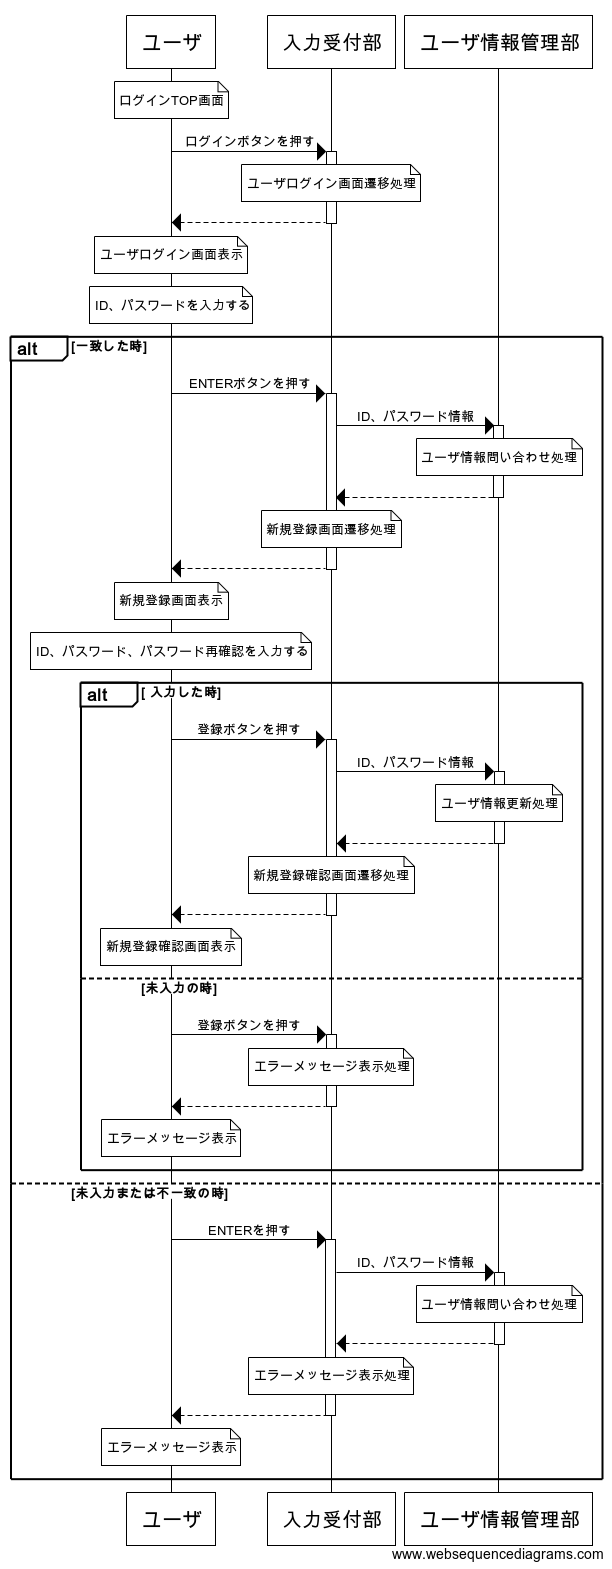
\includegraphics{subsystem/account_new-account.png}}
    \caption{新規登録機能のシーケンス図}
    \label{fig:account_new-account.png}
  \end{figure}
  \subsection{ログインサブシステム(ユーザ用)}
  ログインサブシステムではユーザが設定したIDとパスワードを入力を行う。ログイン時にデータベース登録されているIDとパスワードの認証を行い一致すれば自分のアカウントにログインをすることできる。\\
  ログインサブシステムの機能は小節で示す。
  \subsubsection{ユーザ認証機能}
  ユーザ認証機能では本システムを利用するユーザが、本学の在学生であるかの認証を、IDとパスワードを用いて行う。認証に成功したユーザは、本システムの正当なユーザとして本システムを利用することができる。ユーザ認証機能のシーケンス図は図\ref{fig:login_user.png}に示す。
  \begin{figure}[H]
    \centering
    \resizebox{14cm}{!}{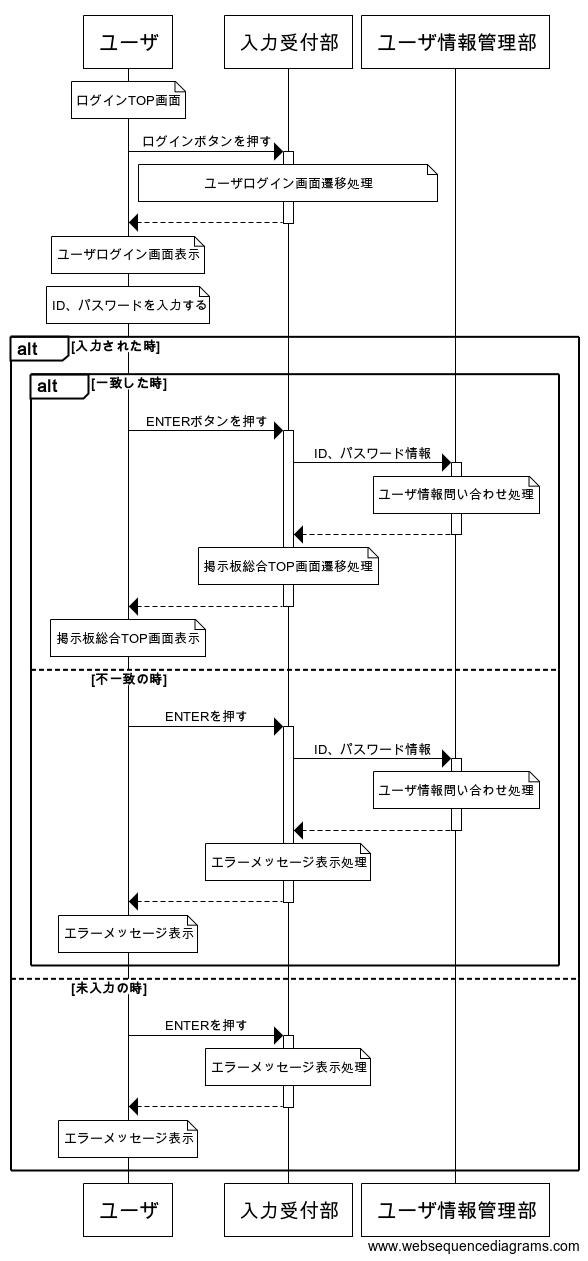
\includegraphics{subsystem/login_user.png}}
    \caption{ユーザ認証機能のシーケンス図}
    \label{fig:login_user.png}
  \end{figure}
  \subsubsection{ログインボーナス機能}
  ログインボーナス機能ではユーザが本システムにログインしたとき、拡張機能と交換できるポイントが付与される。ポイントが付与される頻度は、1日1回に設定している。1回で付与されるポイント数は10ポイントである。ログインボーナス機能のシーケンス図は図\ref{fig:login_login-bonus.png}に示す。
  \begin{figure}[H]
    \centering
    \resizebox{14cm}{!}{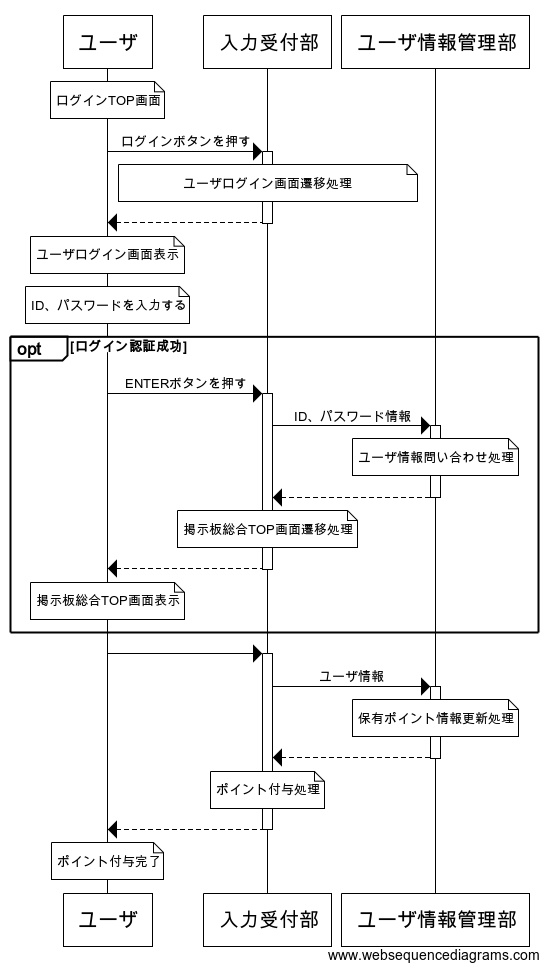
\includegraphics{subsystem/login_login-bonus.png}}
    \caption{ログインボーナス機能のシーケンス図}
    \label{fig:login_login-bonus.png}
  \end{figure}
  \subsubsection{ログアウト機能}
  ログアウト機能ではユーザが本システムにログインしている状態であるとき、「ログアウト」ボタンを押すことで本システムからログアウトすることができる。ログアウト機能のシーケンス図は図\ref{fig:login_logout.png}に示す。
  \begin{figure}[H]
    \centering
    \resizebox{14cm}{!}{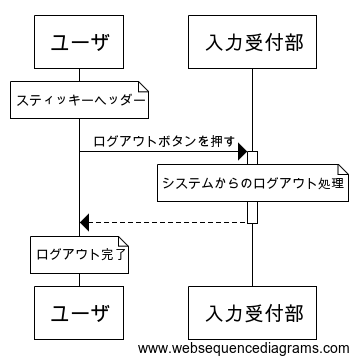
\includegraphics{subsystem/login_logout.png}}
    \caption{ログアウト機能のシーケンス図}
    \label{fig:login_logout.png}
  \end{figure}
  \subsection{検索サブシステム(ユーザ用)}
  検索サブシステムではカテゴリ検索・キーワード検索においてカテゴリを選択、もしくはテキストを入力されたキーワードに該当するスレッドの一覧を表示することができる。\\
  検索サブシステムの機能は小節で示す。
  \subsubsection{検索機能}
  検索機能では所定の検索テキストボックスに任意の文字列を入力し、その文字列に関連したスレッドを一覧で表示することができる。検索方法はand検索、or検索が使用可能である。
  検索機能のシーケンス図は図\ref{fig:search_keyword.png}に示す。
  \begin{figure}[H]
    \centering
    \resizebox{14cm}{!}{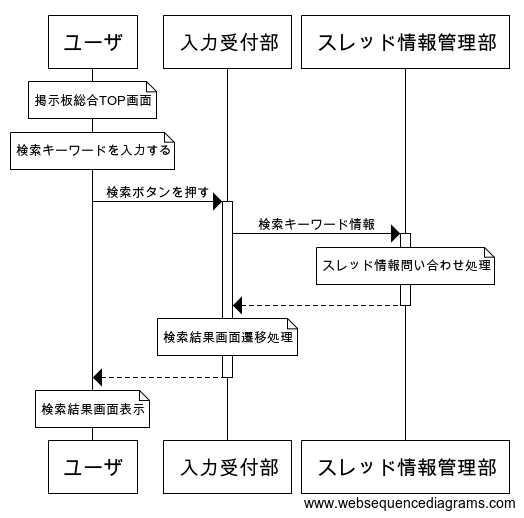
\includegraphics{subsystem/search_keyword.png}}
    \caption{検索機能のシーケンス図}
    \label{fig:search_keyword.png}
  \end{figure}
  \subsubsection{カテゴリ選択機能}
  カテゴリ選択機能では所定の検索テキストボックスの横に設置されたカテゴリ選択ボタンで特定のカテゴリを選択すると、選択されたカテゴリ内に存在するスレッドの中から検索することができる。また、スティキーヘッダーからカテゴリ検索を行うこともできる。
  カテゴリ選択機能のシーケンス図は図に\ref{fig:search_category.png}示す。
  \begin{figure}[H]
    \centering
    \resizebox{14cm}{!}{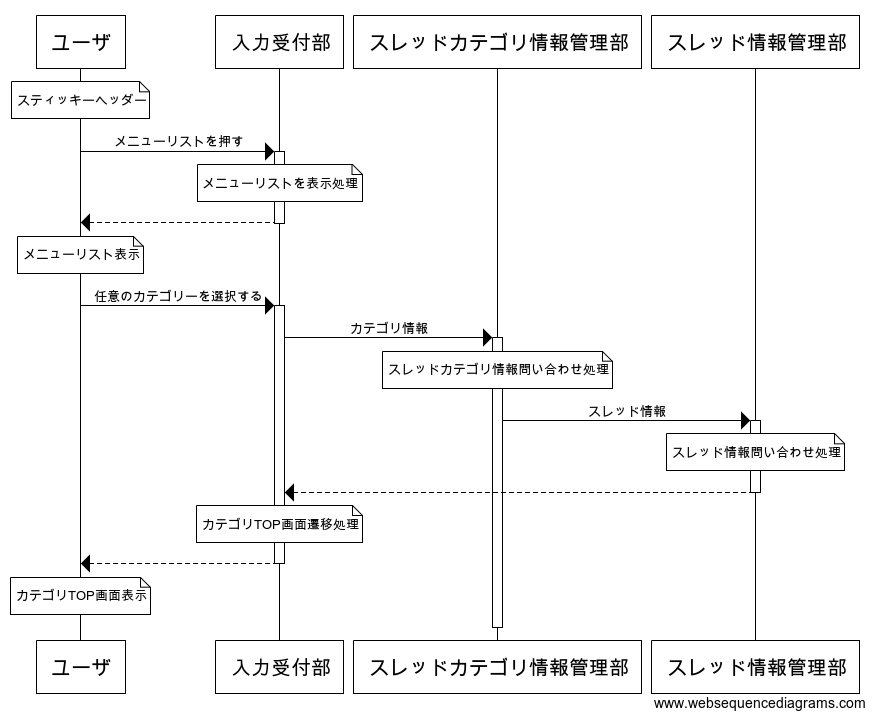
\includegraphics{subsystem/search_category.png}}
    \caption{カテゴリ選択機能のシーケンス図}
    \label{fig:search_category.png}
  \end{figure}
  \subsection{掲示板サブシステム(ユーザ用)}
  掲示板サブシステムではユーザがスレッドの作成・レスの書き込みを行うことができる。\\
  掲示板サブシステムの機能は小節で示す。
  \subsubsection{スレッド作成機能}
  スレッド作成機能ではユーザがスレッドタイトルと最初のレスを入力して、新規のスレッドを作成することができる。
  スレッド作成機能のシーケンス図は図\ref{fig:bbs_thread.png}に示す。
  \begin{figure}[H]
    \centering
    \resizebox{14cm}{!}{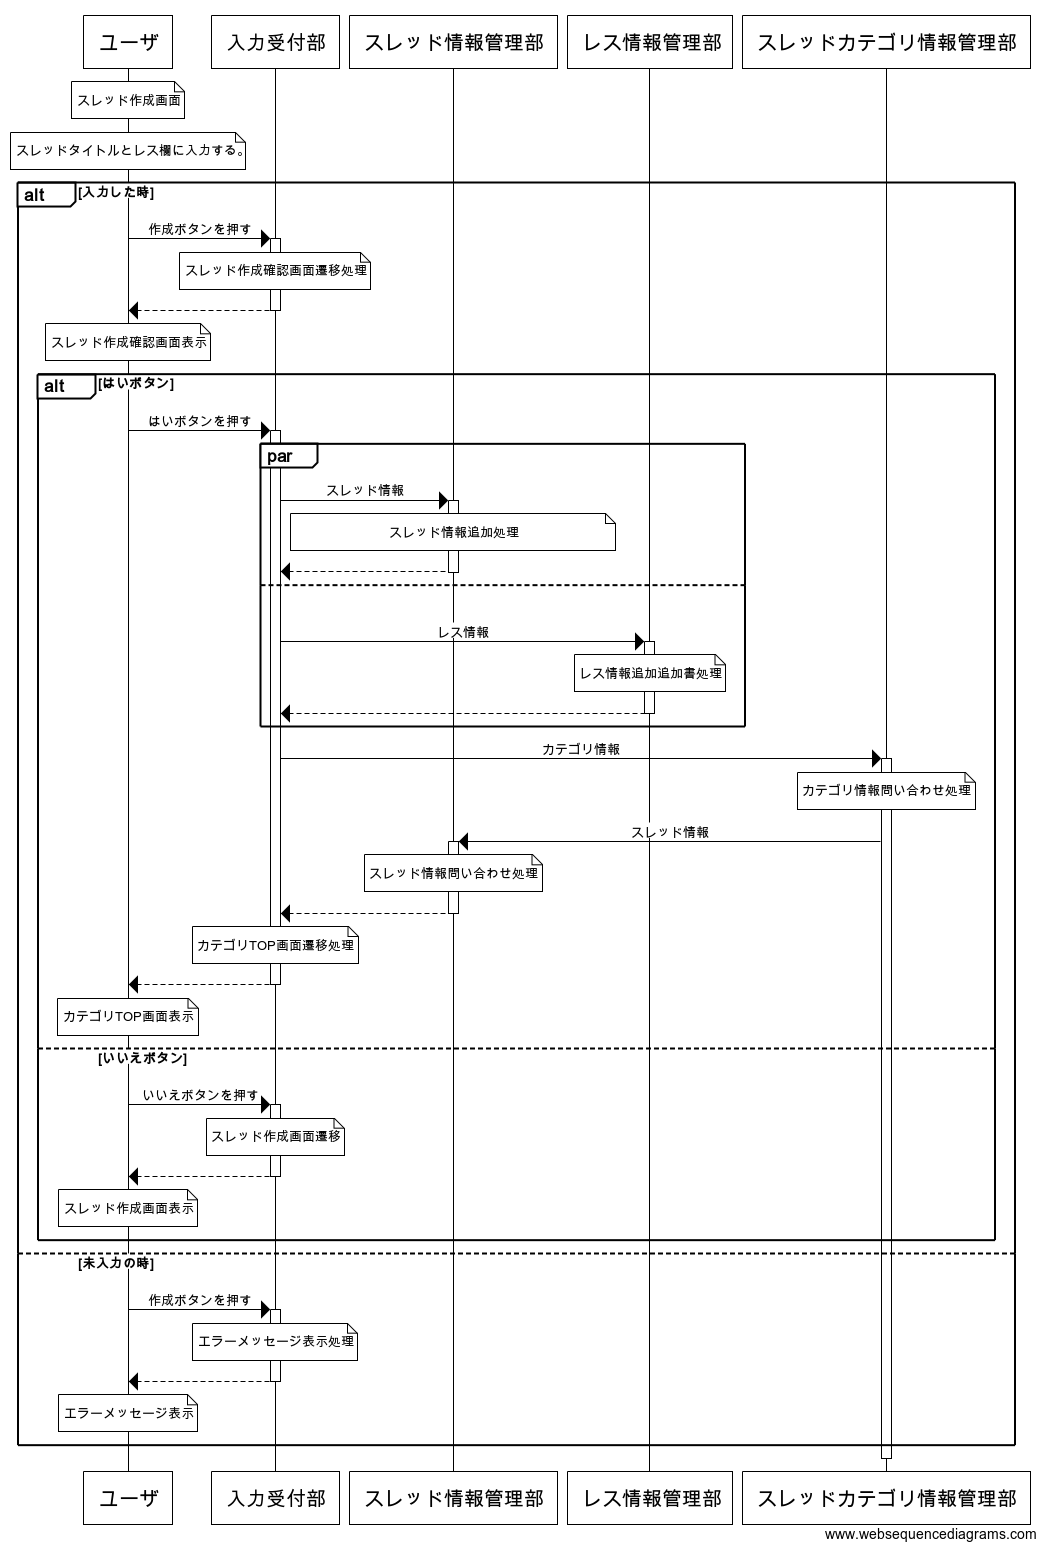
\includegraphics{subsystem/bbs_thread.png}}
    \caption{スレッド作成機能のシーケンス図}
    \label{fig:bbs_thread.png}
  \end{figure}
  \subsubsection{レス書き込み機能}
  レス書き込み機能では既存のスレッド内に、レスを書き込むことができる。このとき、レス番号・ハンドルネーム・日付・レスIDが表示される。レスの書き込み主がハンドルネームを設定している場合、そのハンドルネームが表示される。
  レス書き込み機能のシーケンス図は図に\ref{fig:bbs_res.png}示す。
  \begin{figure}[H]
    \centering
    \resizebox{14cm}{!}{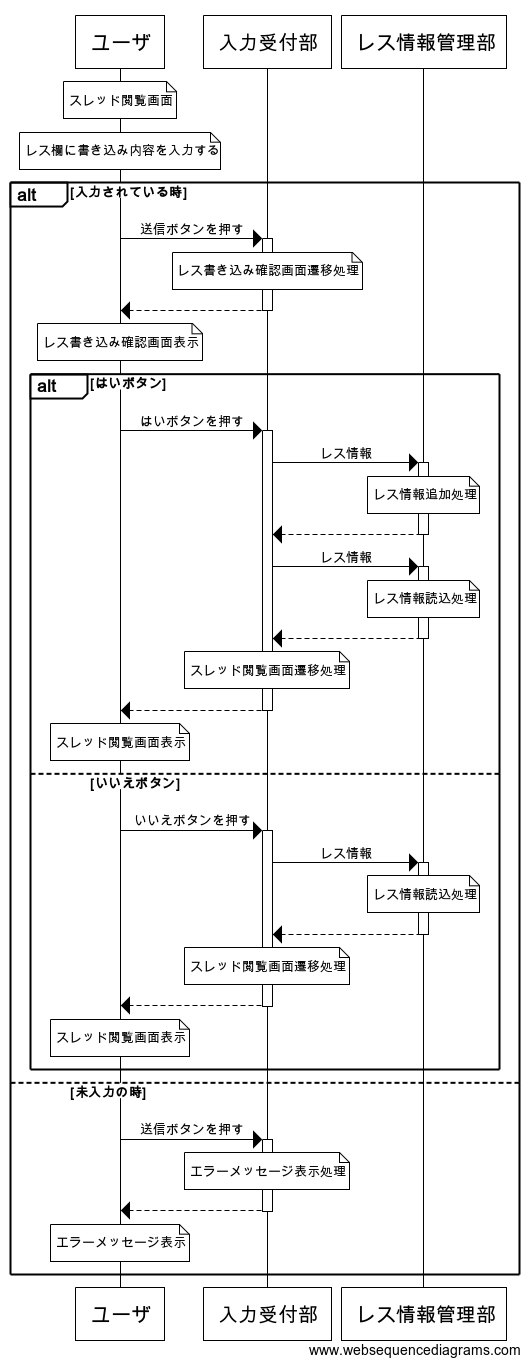
\includegraphics{subsystem/bbs_res.png}}
    \caption{レス書き込み機能のシーケンス図}
    \label{fig:bbs_res.png}
  \end{figure}
  \subsection{お知らせサブシステム(ユーザ用)}
  管理者からユーザに向けて通知されたお知らせ情報を閲覧することができる。\\
  お知らせサブシステムの機能は小節で示す。
  \subsubsection{お知らせ閲覧機能}
  お知らせ閲覧機能では管理者から通達されたお知らせを閲覧することができる。
  お知らせ閲覧機能のシーケンス図は図に\ref{fig:news_reading.png}示す。
  
  \begin{figure}[H]
    \centering
    \resizebox{14cm}{!}{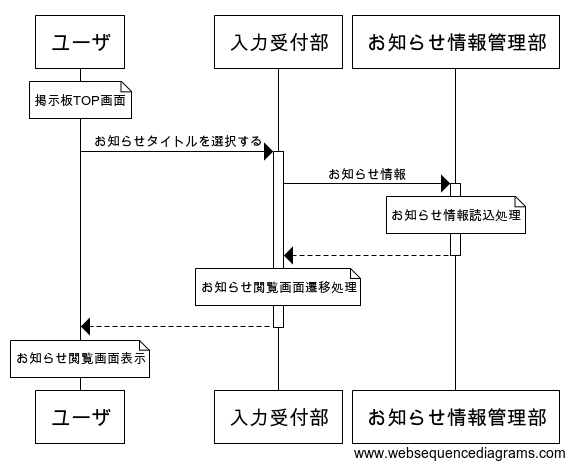
\includegraphics{subsystem/news_reading.png}}
    \caption{お知らせ閲覧機能のシーケンス図}
    \label{fig:news_reading.png}
  \end{figure}
  \subsection{通報サブシステム(ユーザ用)}
  通報サブシステムでは、誹謗中傷や公序良俗に違反してると考えれるスレッドやレスを管理者に通知することができる。\\
  通報サブシステムの機能は小節で示す。
  \subsubsection{スレッド・レス通報機能}
  スレッド・レス通報機能ではユーザが誹謗中傷や公序良俗に違反するなどの不適切な内容であると判断したスレッドまたはレスを管理者に通報することができる。このとき、通報者は通報理由を明記する。
  スレッド・レス通報機能のシーケンス図は図()に示す。
  \subsection{コレクトボタンサブシステム(ユーザ用)}
  コレクトボタンサブシステムでは、ユーザがレスの内容に対して確からしいと判断した際にコレクトボタンを押すことで、コレクト認定(信頼性の認定)をすることができる。\\
  コレクトボタンサブシステムの機能は小節で示す。
  \subsubsection{コレクト認定機能}
  コレクト認定機能ではユーザが特定のレスに対して、その内容が確からしいと判断した場合、コレクトボタンを押してコレクト認定をすることができる。レスの傍らにコレクト認定された回数が表示されるため、コレクト認定は、ユーザがそのレスの内容が確からしいと判断した指標となる。よって、コレクト認定された回数が多いレスは、信憑性のある情報として、ユーザの情報の取捨選択の判断材料となる。なお、1つのレスに対してコレクト認定できる回数は1回のみであり、コレクトボタンを偶数回押すと、コレクト認定を解除することができる。
  コレクト認定機能のシーケンス図は図()に示す。
  \subsubsection{ポイント獲得機能}
  ポイント獲得機能ではユーザが書き込んだレスに他のユーザからコレクト認定された場合、レスの書き込み主は拡張機能を解放するためのポイントを獲得することができる。拡張機能とは、スレッドでレスを行う際にレスの表示が変化する機能である。
  ポイント獲得の相場は、1回のコレクト認定につき1ポイントである。1つのレスにおいて、1人のユーザからポイント獲得できる回数は1回のみである(2回目以降のコレクト認定はポイント獲得できない)。また、コレクト認定が解除されたとしても獲得済のポイントが減ることはない。
  ポイント獲得機能のシーケンス図は図()に示す。
  \subsection{マイページサブシステム(ユーザ用)}
  マイページサブシステムでは、スティッキーヘッダによって表示されているマーク部分を押すことでユーザ情報・ブックマーク閲覧・拡張機能・通知機能を設定することができる。\\
  マイページサブシステムの機能は小節で示す。
  \subsubsection{ユーザ情報設定機能}
  ユーザ情報設定機能ではユーザのハンドルネームの設定ができる。ハンドルネームが設定されていない場合は、「名無し」と表示される。
  ユーザ情報設定機能のシーケンス図は図()に示す。
  \subsubsection{ブックマーク閲覧機能}
  ブックマーク閲覧機能では登録したブックマークの一覧を表示することができる。その中から、任意のスレッドに遷移することができる。
  ブックマーク閲覧機能のシーケンス図は図()に示す。
  \subsubsection{拡張機能}
  拡張機能では本システムを利用して得られたポイントと引き換えに、拡張機能が使用可能となる。主な拡張機能としては、取り消し線、太文字、赤字、斜体などが存在する。1つの拡張機能につき、600ポイントを引き換えると想定する。拡張機能は、今後の仕様変更で追加する可能性がある。
  拡張機能のシーケンス図は図()に示す。
  \subsubsection{通知設定機能}
  通知設定機能では通知機能のON/OFFの設定をすることができる。
  通知設定機能のシーケンス図は図()に示す。
  \subsection{通知サブシステム(ユーザ用)}
  通知サブシステムでは、各ユーザに対してスレッドの書き込み・レスへの返信があった際に処理を行う。
  通知サブシステムの機能は小節で示す。
  \subsubsection{通知機能}
  通知機能ではユーザが作成したスレッドに新たな書き込みがあった場合、またはユーザが書き込んだレスに対して返信が書き込まれた場合に、その旨を通知する。
  通知機能のシーケンス図は図()に示す。
  \subsection{ブックマークサブシステム(ユーザ用)}
  任意のスレッドをブックマークとして登録する際と解除する際に押すことで処理が行われる。
  ブックマークサブシステムの機能は小節で示す。
  \subsubsection{ブックマーク登録機能}
  ブックマーク登録機能では任意のスレッドをブックマークとしてマイページに登録することができる。
  ブックマーク登録機能のシーケンス図は図()に示す。
  \subsubsection{ブックマーク解除機能}
  ブックマーク解除機能ではマイページに存在する任意のブックマークの登録を解除することができる。
  ブックマーク解除機能のシーケンス図は図()に示す。
  \subsection{子管理者管理サブシステム(管理者用)}
  子管理者サブシステムでは親管理者が子管理者のアカウントを管理するサブシステムである。親管理者がIDとパスワードを発行することで、本システムを管理する子管理者を登録することができる。また、不要になった子管理者のアカウントを抹消することがきる。\\
  子管理者管理サブシステムの機能は小節で示す。
  \subsubsection{子管理者用ID・パスワード発行機能}
  子管理者用ID・パスワード発行機能では親管理者は手動で子管理者のIDとパスワードを登録し、発行することができる。子管理者にはこの機能は存在しない。子管理者用ID・パスワード発行機能のシーケンス図は図\ref{fig:admin_children_id-pass.png}に示す。
  \begin{figure}[H]
    \centering
    \resizebox{14cm}{!}{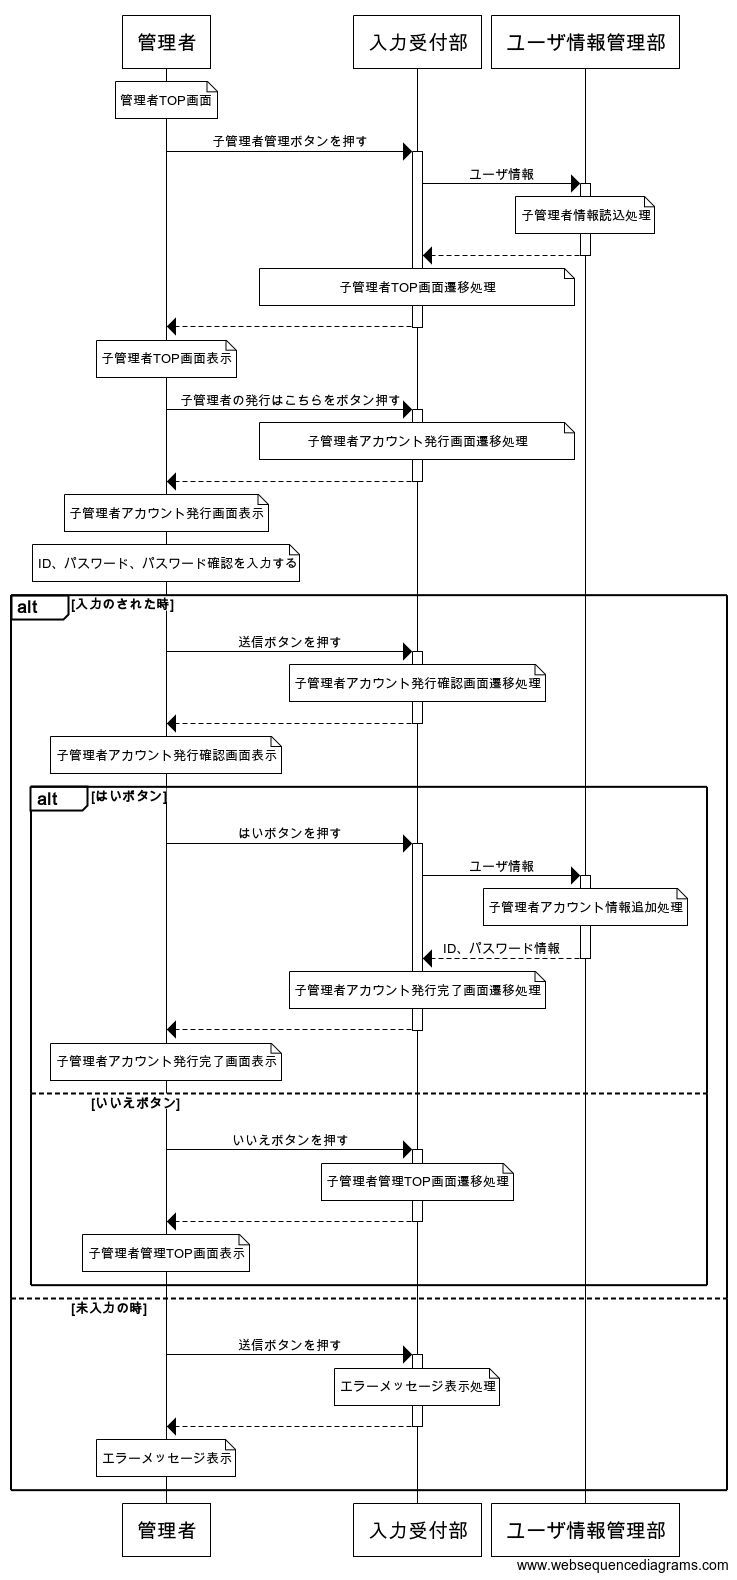
\includegraphics{subsystem/admin_children_id-pass.png}}
    \caption{子管理者用ID・パスワード発行機能のシーケンス図}
    \label{fig:admin_children_id-pass.png}
  \end{figure}
  
  \subsubsection{子管理者アカウント抹消機能}
  子管理者アカウント抹消機能では親管理者は手動で不要になった子管理者のアカウントを抹消することができる。子管理者アカウント抹消機能のシーケンス図は図\ref{fig:admin_children-delete.png}に示す。
  \begin{figure}[H]
    \centering
    \resizebox{14cm}{!}{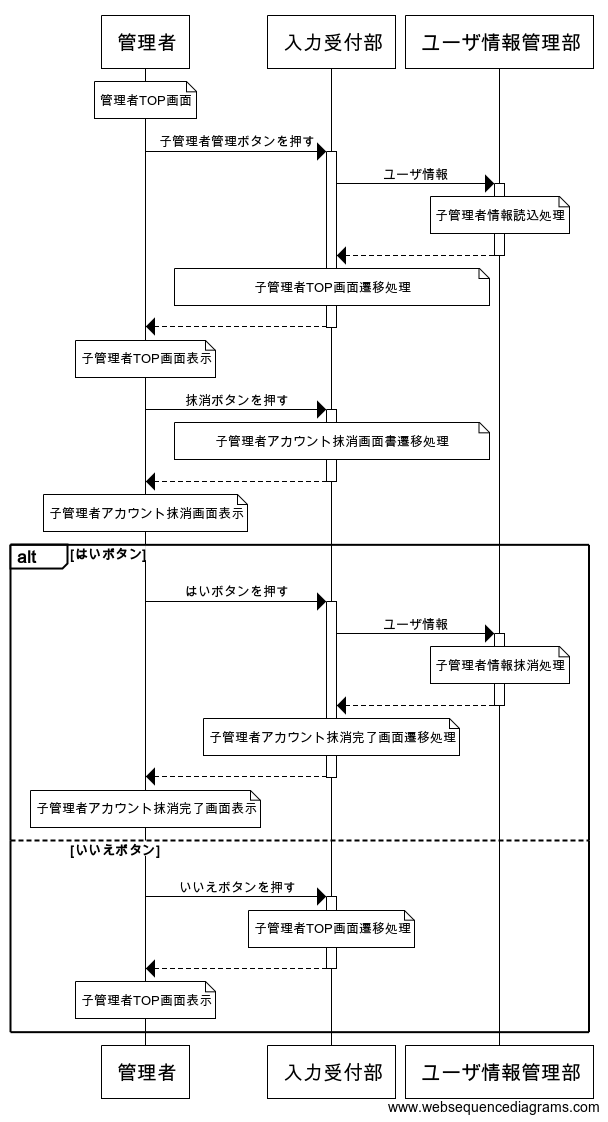
\includegraphics{subsystem/admin_children-delete.png}}
    \caption{子管理者アカウント抹消機能のシーケンス図}
    \label{fig:admin_children-delete.png}
  \end{figure}
  
  \subsubsection{子管理者情報閲覧機能}
  子管理者情報閲覧機能では親管理者は子管理者のIDとパスワードを閲覧することができる。子管理者情報閲覧機能のシーケンス図は図\ref{fig:admin_children-reading.png}に示す。
  \begin{figure}[H]
    \centering
    \resizebox{14cm}{!}{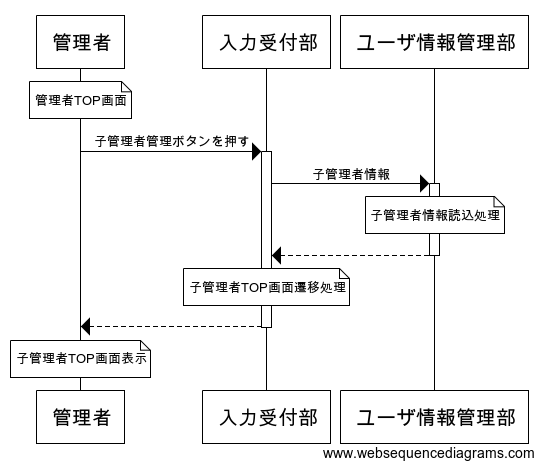
\includegraphics{subsystem/admin_children-reading.png}}
    \caption{子管理者情報閲覧機能のシーケンス図}
    \label{fig:admin_children-reading.png}
  \end{figure}
  \subsection{お知らせ編集サブシステム(管理者用)}
  お知らせ編集サブシステムでは管理者からユーザ全体に対して任意のお知らせを通達することができる。\\
  お知らせ編集サブシステムの機能は小節で示す。
  \subsubsection{お知らせ編集機能}
  お知らせ編集機能では管理者は、ユーザに対して通達するお知らせタイトルとその内容を編集することができる。お知らせ編集機能のシーケンス図は図\ref{fig:admin_news.png}に示す。
  \begin{figure}[H]
    \centering
    \resizebox{14cm}{!}{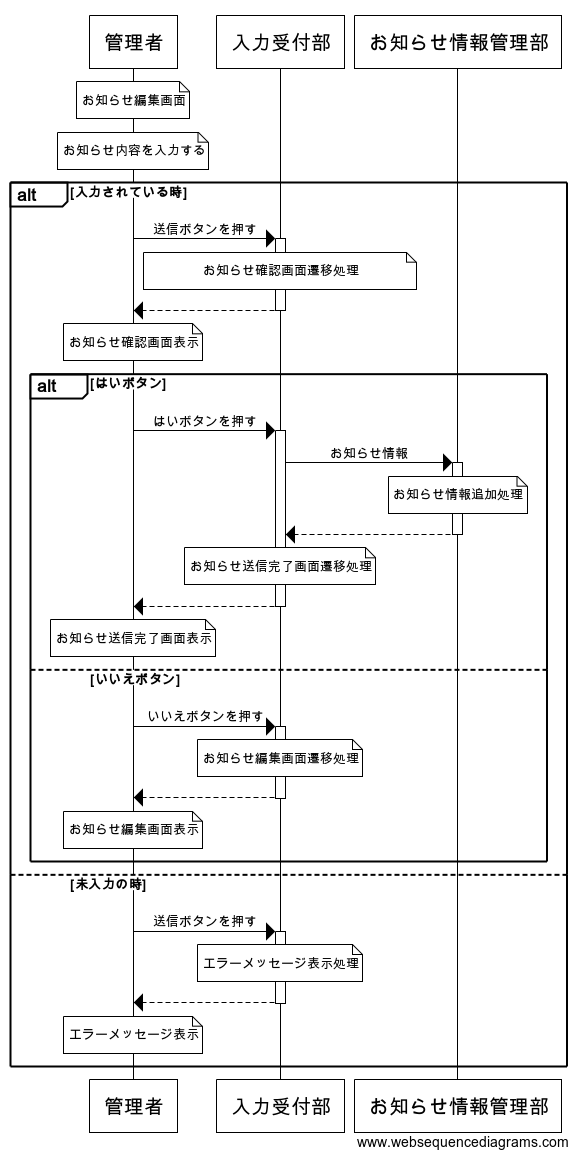
\includegraphics{subsystem/admin_news.png}}
    \caption{お知らせ編集機能のシーケンス図}
    \label{fig:admin_news.png}
  \end{figure}
  \subsubsection{お知らせ表示機能}
  お知らせ表示機能本システムのトップページに、お知らせ編集機能で編集した日付とタイトルを表示することができる。お知らせ表示機能のシーケンス図は図\ref{fig:admin_news_display.png}に示す。
  \begin{figure}[H]
    \centering
    \resizebox{14cm}{!}{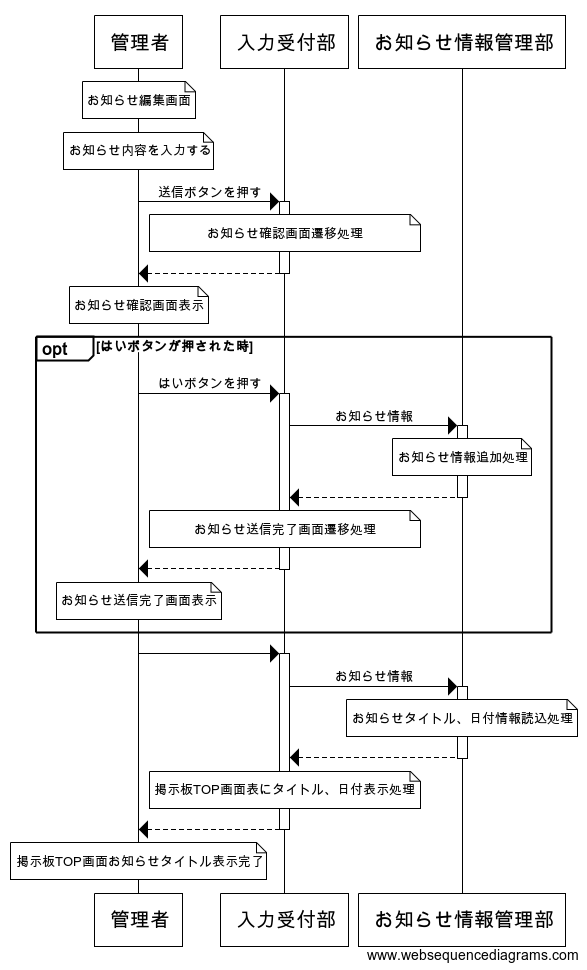
\includegraphics{subsystem/admin_news_display.png}}
    \caption{お知らせ表示機能のシーケンス図}
    \label{fig:admin_news_display.png}
  \end{figure}
  \subsubsection{お知らせリンク機能}
  お知らせ編集機能で編集したお知らせ内容を本システムトップページに表示されているお知らせタイトルにリンクを追加することができる。
  \subsection{掲示板編集サブシステム(管理者用)}
  掲示板編集サブシステムでは管理者は不適切であると判断したスレッドやレスを非表示することができる。また、不適切な単語を登録することで自動置換する。ユーザから送られてきたスレッドやレスに対しての通報内容を閲覧することもできる。\\
  掲示板編集サブシステムの機能は小節で示す。
  \subsubsection{スレッド非表示化機能}
  スレッド非表示化機能は管理者が、データベースに存在するスレッド及びスレッドに格納された全てのレスを非表示化することができる。スレッド非表示化機能のシーケンス図は図 \ref{fig:admin_bbs_thread-hide.png} に示す。
  \begin{figure}[H]
    \centering
    \resizebox{14cm}{!}{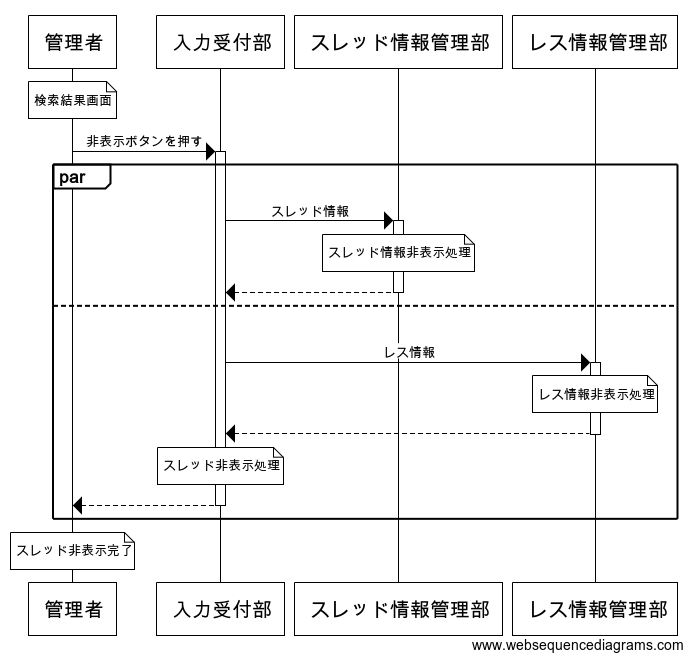
\includegraphics{subsystem/admin_bbs_thread-hide.png}}
    \caption{スレッド非表示化機能のシーケンス図}
    \label{fig:admin_bbs_thread-hide.png}
  \end{figure}
  \subsubsection{レス非表示化機能}
  レス非表示化機能では管理者が、データベースに存在するスレッド内のレスを非表示化することができる。レス非表示化機能のシーケンス図は図 \ref{fig:admin_bbs_res-hide.png} に示す。
  \begin{figure}[H]
    \centering
    \resizebox{14cm}{!}{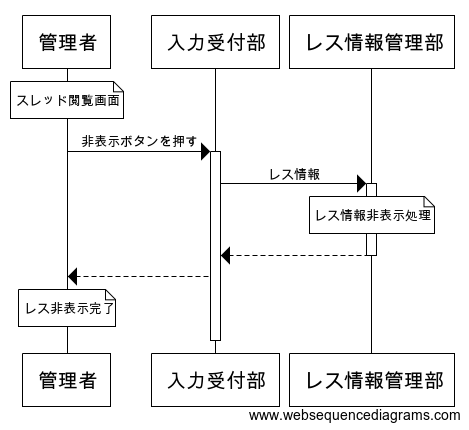
\includegraphics{subsystem/admin_bbs_res-hide.png}}
    \caption{レス非表示化機能のシーケンス図}
    \label{fig:admin_bbs_res-hide.png}
  \end{figure}
  \subsection{非表示化履歴閲覧機能}
  非表示化履歴閲覧機能では管理者は、非表示化したスレッドまたはレスを一覧で閲覧することができる。非表示化履歴閲覧機能のシーケンス図は図 \ref{fig:admin_bbs_hide-history.png} に示す。
  \begin{figure}[H]
    \centering
    \resizebox{14cm}{!}{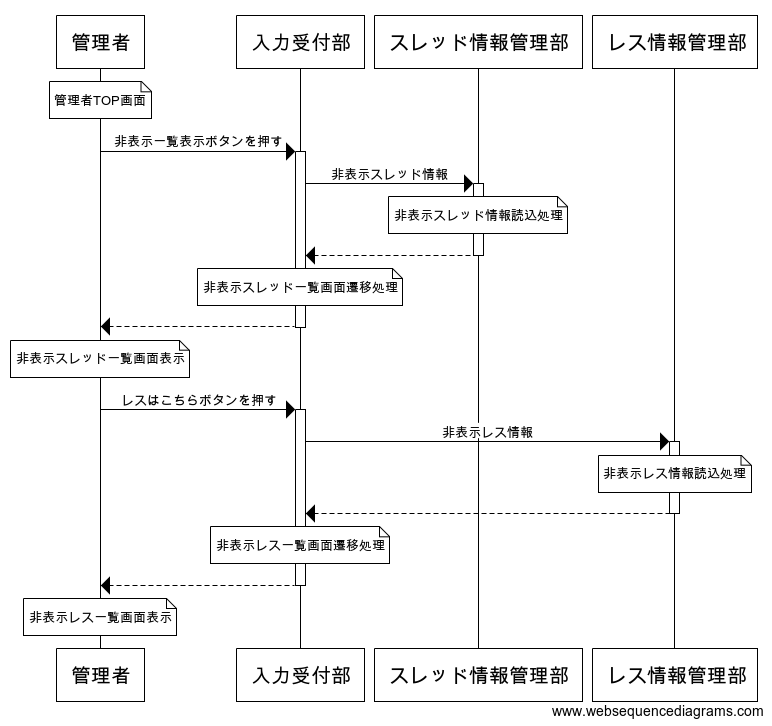
\includegraphics{subsystem/admin_bbs_hide-history.png}}
    \caption{非表示化履歴閲覧機能のシーケンス図}
    \label{fig:admin_bbs_hide-history.png}
  \end{figure}
  \subsubsection{不適切な単語登録機能}
  不適切な単語登録機能では管理者が、誹謗中傷や公序良俗に違反していると考えられる単語を登録することができる。不適切な単語登録機能のシーケンス図は図 \ref{fig:admin_bbs_wordentry.png} に示す。
  \begin{figure}[H]
    \centering
    \resizebox{14cm}{!}{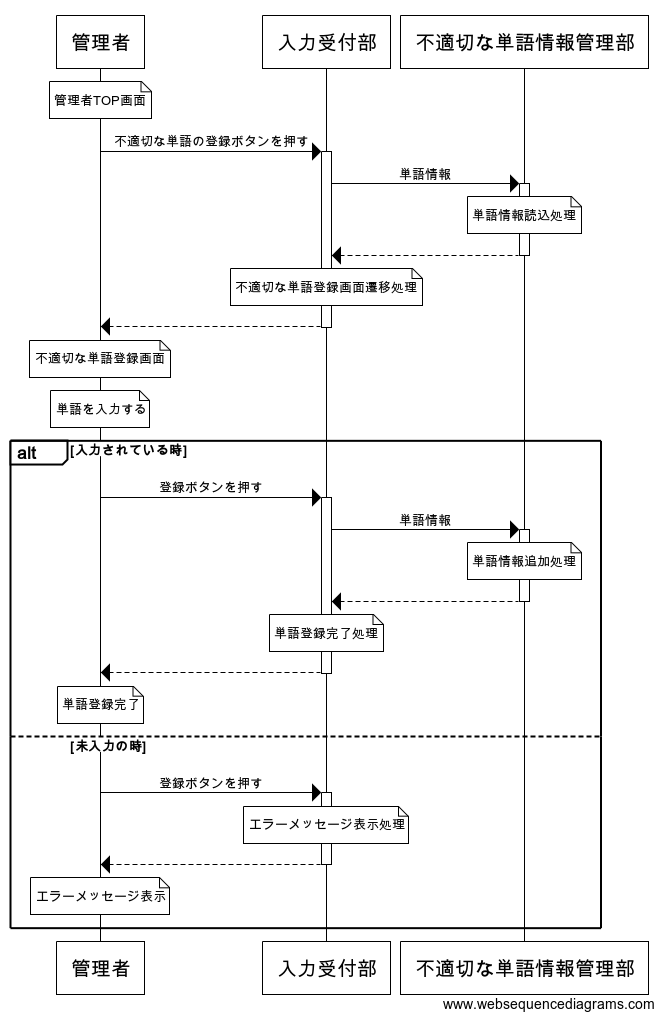
\includegraphics{subsystem/admin_bbs_wordentry.png}}
    \caption{不適切な単語登録機能のシーケンス図}
    \label{fig:admin_bbs_wordentry.png}
  \end{figure}
  \subsubsection{不適切な単語自動置換機能}
  不適切な単語自動置換機能では管理者が設定した不適切な単語を検出し次第、自動で伏せ字に置換することができる。不適切な単語自動置換機能のシーケンス図は、図 \ref{fig:admin_bbs-replace.png} に不適切な単語登録機能で単語登録された時に不適切な単語を検出した場合について示し、図 \ref{fig:admin_bbs_replace-res.png} にユーザがレス書き込みを行った場合に不適切な単語を含んでいた場合について示す。
  \begin{figure}[H]
    \centering
    \resizebox{14cm}{!}{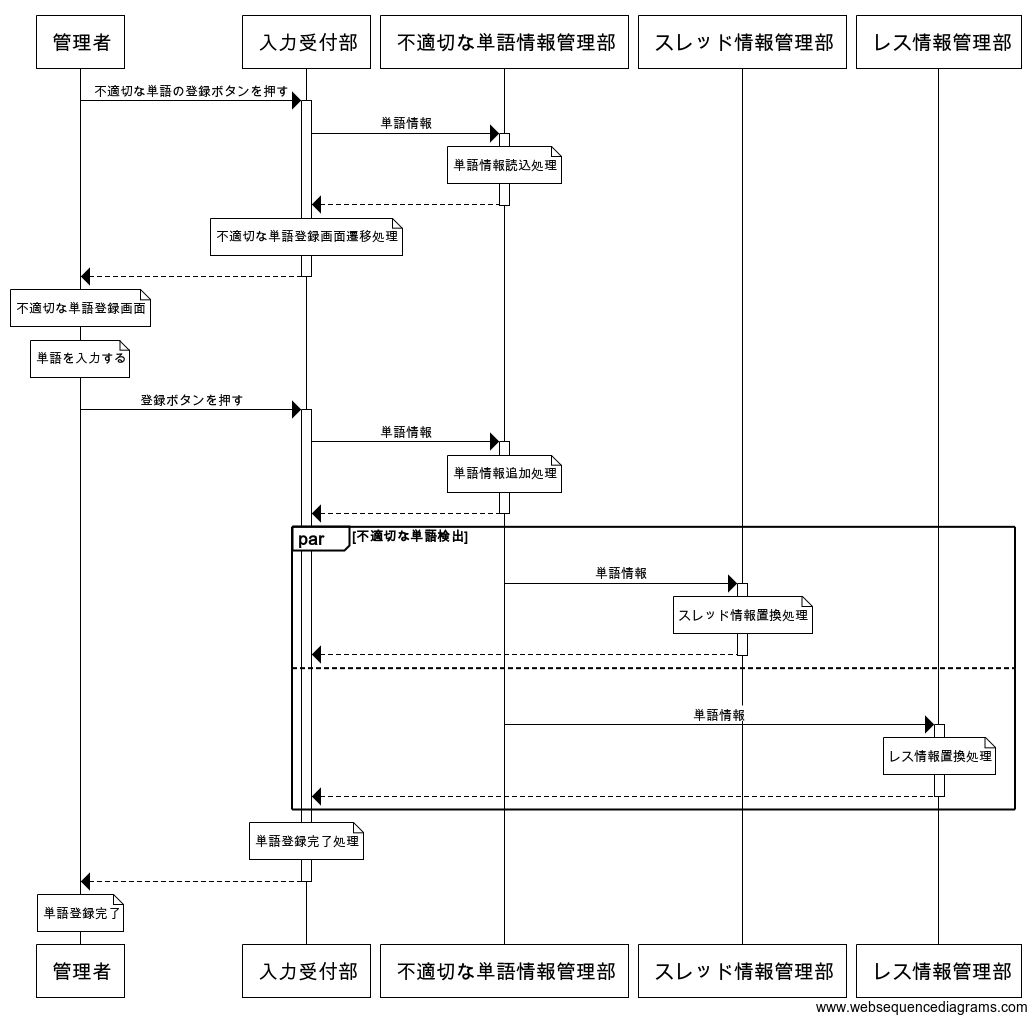
\includegraphics{subsystem/admin_bbs-replace.png}}
    \caption{不適切な単語自動置換機能のシーケンス図(不適切な単語を検出した時)}
    \label{fig:admin_bbs-replace.png}
  \end{figure}
  
  \begin{figure}[H]
    \centering
    \resizebox{14cm}{!}{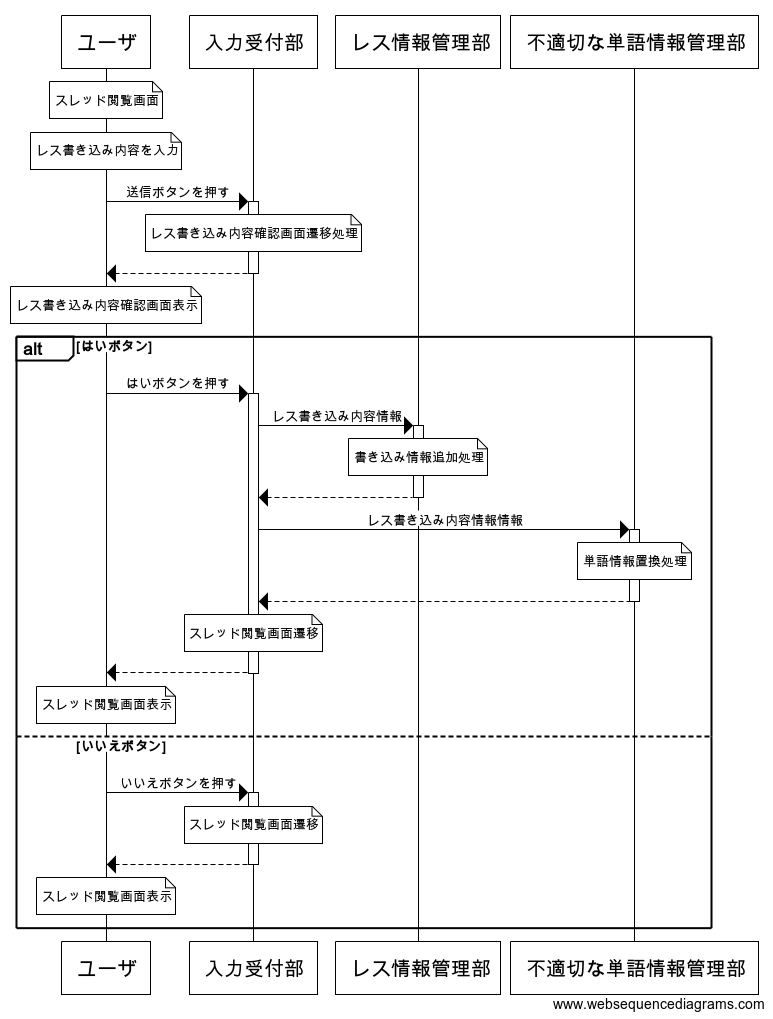
\includegraphics{subsystem/admin_bbs_replace-res.png}}
    \caption{不適切な単語自動置換機能のシーケンス図(レス書き込みの時)}
    \label{fig:admin_bbs_replace-res.png}
  \end{figure}
  \subsubsection{通報内容閲覧機能}
  通報内容閲覧機能ユーザによって通報されたスレッドまたはレスの内容の一覧を、通報理由と共に閲覧することができる。このとき、通報者のユーザ情報、通報されたスレッド主またはレスの書き込み主のユーザ情報も同時に表示される。通報内容閲覧機能のシーケンス図は図 \ref{fig:admin_bbs_report-reading.png} に示す。
  \begin{figure}[H]
    \centering
    \resizebox{14cm}{!}{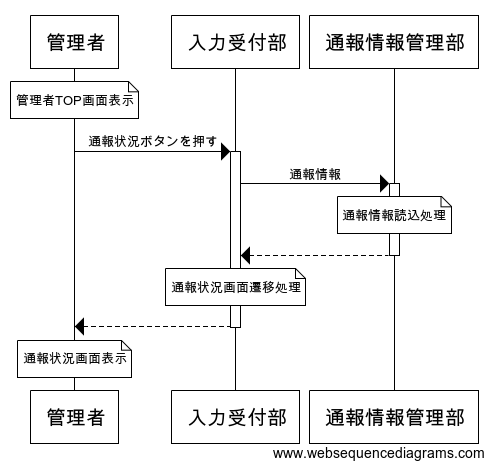
\includegraphics{subsystem/admin_bbs_report-reading.png}}
    \caption{通報内容閲覧機能のシーケンス図}
    \label{fig:admin_bbs_report-reading.png}
  \end{figure}
  \subsection{ユーザ管理サブシステム(管理者用)}
  管理者はユーザの情報を検索し、閲覧することができる。また、不適切なスレッドやレスを書き込んだユーザに対して警告やアカウント凍結などの処置を行うことができる。\\
  ユーザ管理サブシステムの機能は小節で示す。
  \subsubsection{ユーザ情報機能検索機能、ユーザ情報閲覧機能機能}
  ユーザ情報機能検索機能とユーザ情報閲覧機能機能では管理者が、データベースに登録されているユーザ情報の中から特定のユーザ情報を検索しユーザの情報を閲覧することができる。ユーザ情報検索機能とユーザ情報閲覧機能のシーケンス図は図 \ref{fig:admin_user_reading-search.png} に示す。
  \begin{figure}[H]
    \centering
    \resizebox{14cm}{!}{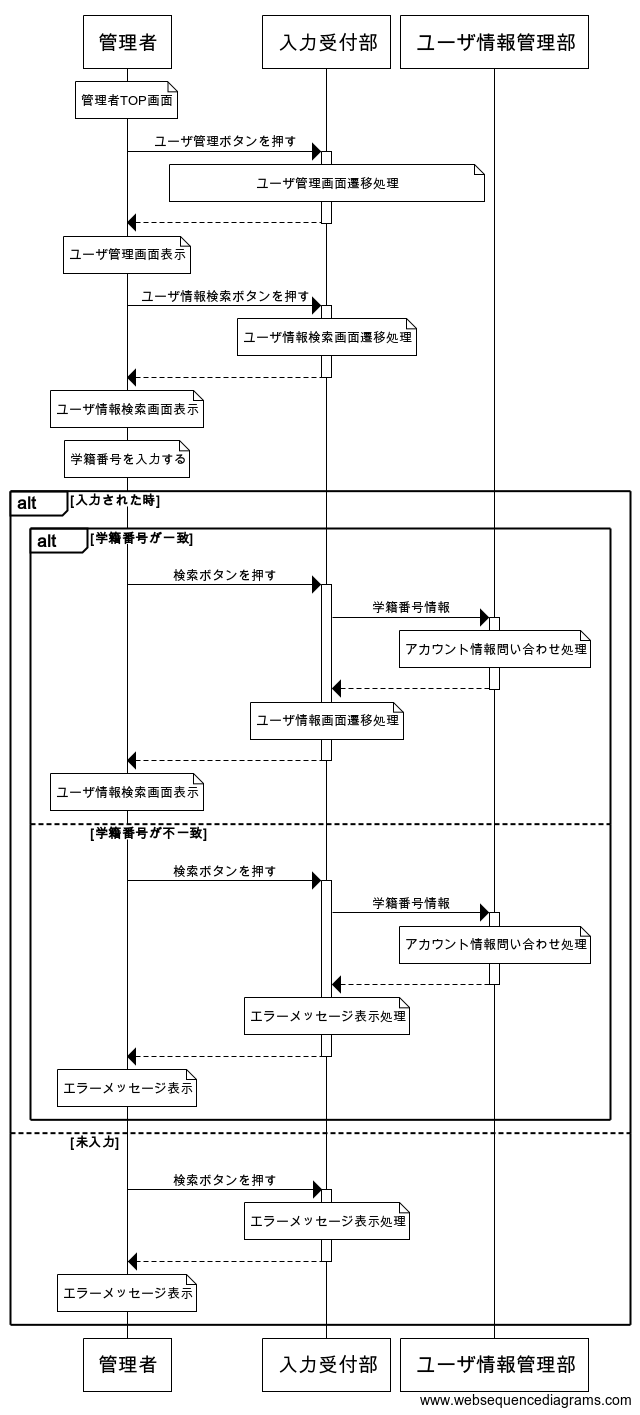
\includegraphics{subsystem/admin_user_reading-search.png}}
    \caption{ユーザ情報機能検索機能とユーザ情報閲覧機能機能のシーケンス図}
    \label{fig:admin_user_reading-search.png}
  \end{figure}
  \subsubsection{ユーザに対する警告通知送信機能}
  ユーザに対する警告通知送信機能では管理者が、不適切な内容のスレッド作成またはレスの書き込みを度々行ったユーザに対して、注意喚起の旨をユーザのマイページに通知することができる。ユーザに対する警告通知送信機能のシーケンス図は図 \ref{fig:admin_user_warning.png} に示す。
  \begin{figure}[H]
    \centering
    \resizebox{14cm}{!}{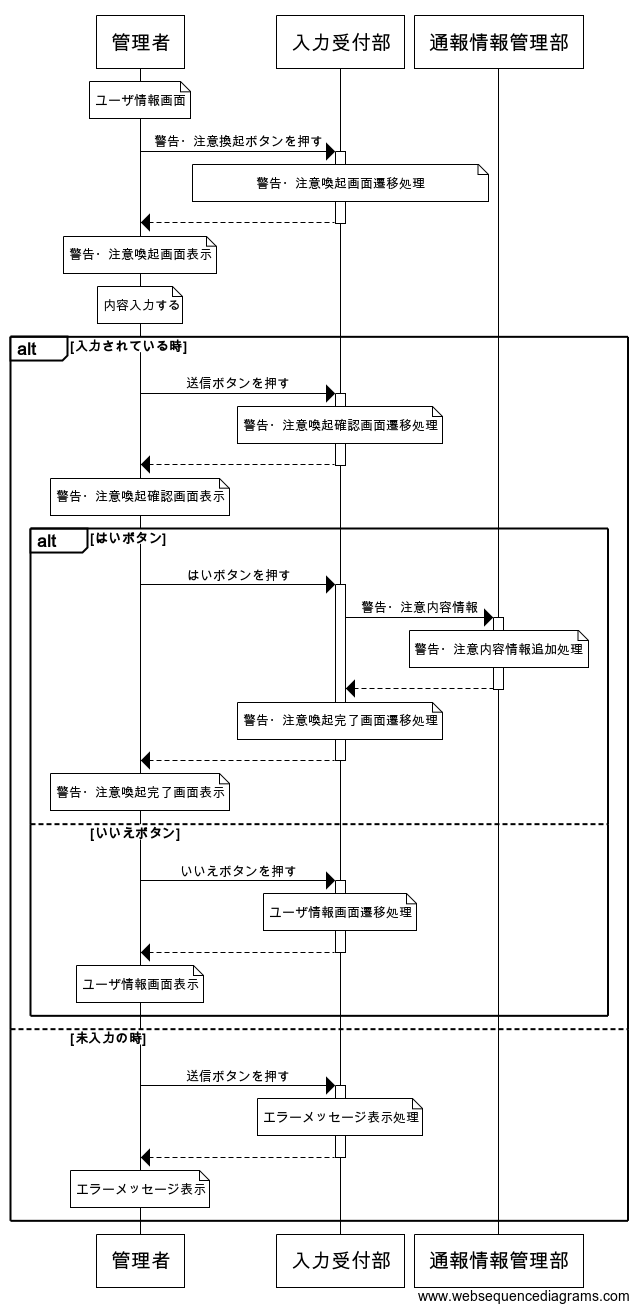
\includegraphics{subsystem/admin_user_warning.png}}
    \caption{ユーザに対する警告通知送信機能のシーケンス図}
    \label{fig:admin_user_warning.png}
  \end{figure}
  \subsubsection{ユーザアカウント凍結機能}
  ユーザアカウント凍結機能管理者が、度重なる注意を通達したにも関わらず、迷惑行為が改善されないユーザのアカウントに対して、書き込み不可能にすることができる。ユーザアカウント凍結機能のシーケンス図は図 \ref{fig:admin_user-suspend.png} に示す。
  \begin{figure}[H]
    \centering
    \resizebox{14cm}{!}{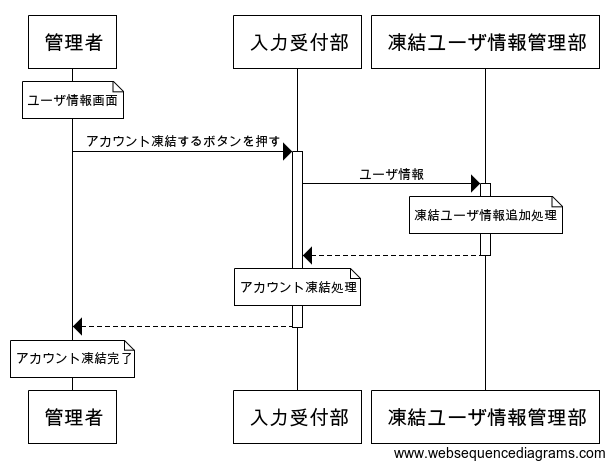
\includegraphics{subsystem/admin_user-suspend.png}}
    \caption{ユーザアカウント凍結機能のシーケンス図}
    \label{fig:admin_user-suspend.png}
  \end{figure}
  \subsection{ユーザ登録サブシステム(管理者用)}
  管理者はユーザの仮IDと仮パスワードの発行を行うことができる。仮IDと仮パスワードを用いて、ユーザは本システムに新規登録することができる。\\
  ユーザ登録サブシステムの機能は小節で示す。
  \subsubsection{仮ID・仮パスワード発行機能}
  仮ID・仮パスワード発行機能では管理者が仮IDと仮パスワードを発行することができる。仮IDと仮パスワードの生成には、乱数を用いる。 仮ID・仮パスワード発行機能のシーケンス図は図 \ref{fig:admin_user_id-pass.png} に示す。
  \begin{figure}[H]
    \centering
    \resizebox{14cm}{!}{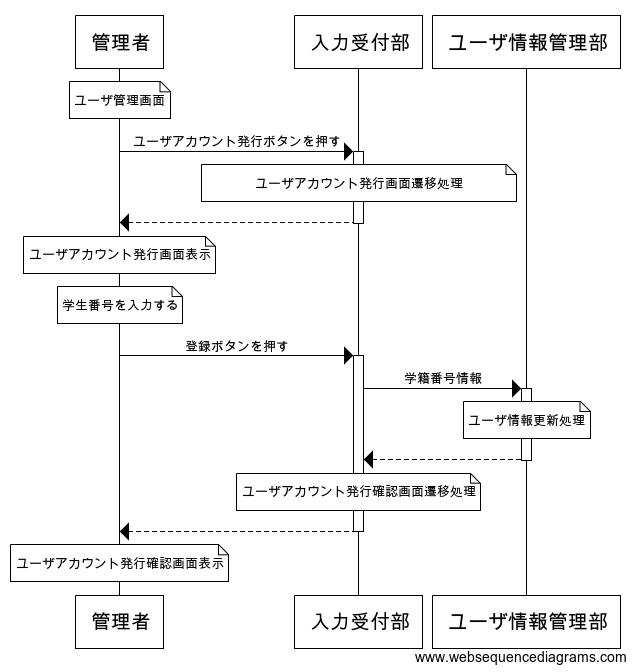
\includegraphics{subsystem/admin_user_id-pass.png}}
    \caption{仮ID・仮パスワード発行機能のシーケンス図}
    \label{fig:admin_user_id-pass.png}
  \end{figure}
  \subsection{管理者ログインサブシステム(管理者用)}
  管理者は学内LANに接続された電子デバイスからのみ、管理者のIDとパスワードを入力することで、管理者として本システムにログインすることができる。\\
  管理者ログインサブシステムの機能は小節で示す。
  \subsubsection{管理者認証機能}
  管理者認証では本システムの管理作業を行うユーザが、管理者であるかの認証を、IDとパスワードを用いて行う。認証に成功したユーザは管理者として本システムの管理を行うことができる。管理者認証機能のシーケンス図は図 \ref{fig:admin_admin-login.png} に示す。
  \begin{figure}[H]
    \centering
    \resizebox{14cm}{!}{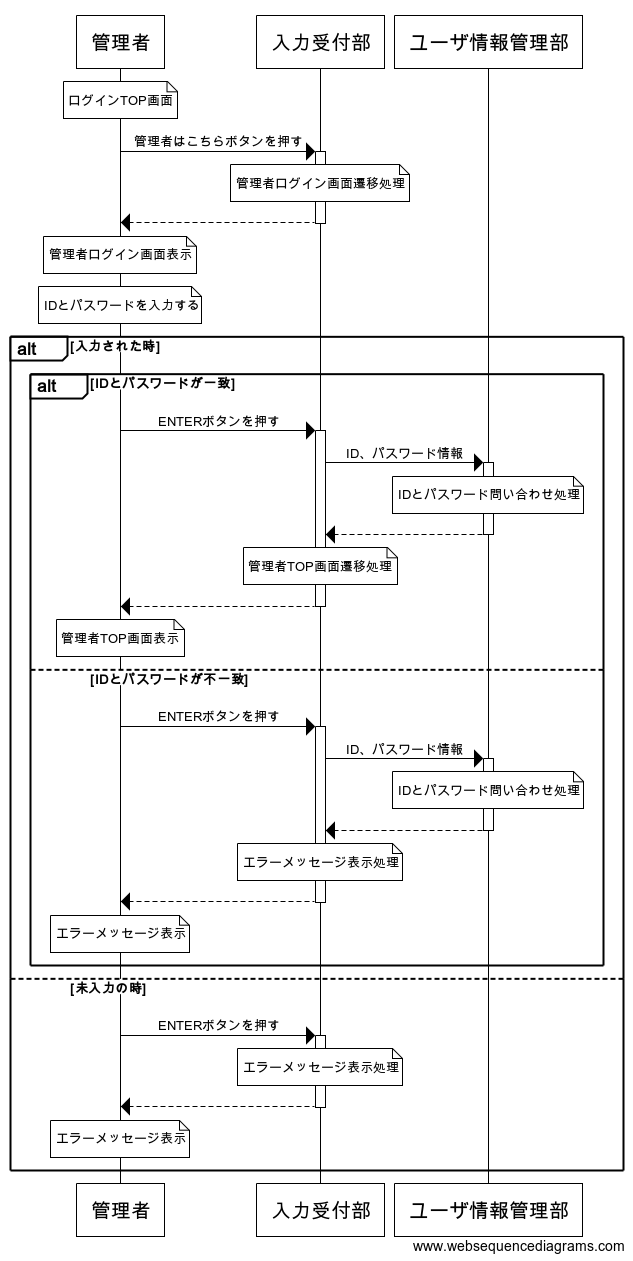
\includegraphics{subsystem/admin_admin-login.png}}
    \caption{管理者認証機能のシーケンス図}
    \label{fig:admin_admin-login.png}
  \end{figure}

\section{ルーティング及びMVC一覧}
この章では、Railsの規約に従ったURL規則を示す。また、HTTPメソッドとURLによって呼び出されるControllerとActionを示す。さらに、View及びModelも示す。
\newpage
\subsection{ルーティング一覧}
以下の表は、Railsの規則に従ったURL規則の表である。また、ControllerとそのActionについても示す。



\begin{table}[htb]
  \caption{ルーティング一覧No.1}
  \centering
  \begin{tabular}{|c|l|l||l|} \hline
   No. & URL & METHOD & Controller\#Action \\ \hline \hline

   1 & /top & GET & top\#home \\ \hline

	 2 & /login & GET & sessions\#new \\
   3 & /login & POST & sessions\#create \\
	 4 & /logout & DELETE & sessions\#destroy \\ \hline

	 5 &	/passwords/:id & GET & passwords\#new \\
	 6 & /passwords/:id	& PATCH	& passwords\#update \\
   7 & /passwords/:id/signup & GET & passwords\#signup \\ \hline

	 8 &	/home	& GET & home\_pages\#home \\ \hline

	 9 &	/users/:id & GET & users\#show \\
	 10 &	/users/:id/name\_update & PATCH & users\#name\_update \\
   11 & /users/:id/notification & PATCH & users\#notification \\
   12 & /users/:id/warning & GET & users\#warning \\
   13 & /users/:id/extension & PATCH & users\#extension \\ \hline

	14 &	/results & GET & results\#search \\ \hline

	15 &	/categories/:id & GET & categories\#index \\ \hline

	16 &	/threads/new  & GET & threads\#new \\
	17 & /threads/check & GET & threads\#check \\
	18 & /threads & POST & threads\#create \\
  19 & /threads/:id & GET & threads\#show \\ \hline

	% 17 & /threads/:id/report\_new & GET & threads\#report\_new \\

	20 & /threads/:id/contents/check	& GET & contents\#check \\
	21 & /threads/:id/contents/create & POST  & contents\#create \\
	22 & /threads/:id/contents/correct & PATCH & contents\#correct \\ \hline

  23 & /threads/:id/report\_form & GET & report\#new \\
  24 & /threads/:id/contents/:id/report\_form & GET & report\#new \\
  25 & /threads/:id/report\_check & GET & report\#check \\
  26 & /threads/:id/contents/:id/report\_check & GET & report\#check \\
  27 & /threads/:id/report & POST & report\#craete \\
  28 & /threads/:id/contents/:id/report & POST & report\#create \\
  29 & /admins/report & GET & report\#index \\ \hline

  30 & /threads/:id/bookmark\_create & POST & bookmark\#create \\
  31 & /threads/:id/bookmark\_destroy & DELETE & bookmark\#destroy \\ \hline

\end{tabular}

\end{table}


\begin{table}[H]
  \centering
  \caption{ルーティング一覧No.2}
  \begin{tabular}{|c|l|l||l|}\hline
    No. & URL & METHOD & Controller\#Action \\ \hline \hline

    32 & /threads/:id/hide & PATCH & hide\#thread\_hide \\
    33 & /threads/:id/contents/:id/hide & PATCH & hide\#res\_hide \\
    34 & /admins/threads/:id/hide & GET & hide\#thread\_index \\
    35 & /admins/threads/:id/contents/:id/hide & GET & hide\#res\_index \\ \hline

    36 & /admins/login & GET & admins\_session\#new \\
    37 & /admins/login & POST & admins\_session\#login \\
    38 & /admins/logout & DELETE & admins\_session\#logout \\ \hline

    39 & /admins/top & GET & admins\_top\#home \\ \hline

    40 & /admins/ng\_word & GET & ng\_word\#home \\
    41 & /admins/ng\_word/create & POST & ng\_word\#create \\
    42 & /admins/ng\_word/destroy & DELETE & ng\_word\#destroy \\ \hline

    43 & /admins/manage & GET & manage\#home \\
    44 & /admins/manage/signup & GET & manage\#signup \\
    45 & /admins/manage/signup & POST & manage\#create \\
    46 & /admins/manage/ok & GET & manage\#ok \\
    47 & /admins/manage/destroy & GET & manage\#destroy\_check \\
    48 & /admins/manage/destroy & DELETE & manage\#destroy \\ \hline

    49 & /admins/manage\_user & GET & manage\_user\#home \\
    50 & /admins/manege\_user/signup & GET & manage\_user\#user\_signup \\
    51 & /admins/manage\_user/signup & POST & manage\_user\#user\_create \\
    52 & /admins/manage\_user/search & GET & manage\_user\#search \\
    53 & /admins/manage\_user/:id & GET & manage\_user\#show \\
    54 & /admins/manage\_user/edit & GET & manage\_user\#warning\_edit \\
    55 & /admins/manage\_user/check & GET & manage\_user\#warning\_check \\
    56 & /admins/manage\_user/create & POST & manage\_user\#warning\_create \\
    57 & /admins/manage\_user/id/ban\_create & PATCH & manage\_user\#ban\_create \\ \hline
    58 & /admins/manage\_user/id/ban\_destroy & PATCH & manage\_user\#ban\_destroy \\ \hline
    59 & /admins/announce & GET & announce\#edit \\
    60 & /admins/announce\_check & GET & announce\#check \\
    61 & /admins/announce\_create & POST & announce\#create \\
    62 & /home/announce/:id & GET & announce\#show \\ \hline
  \end{tabular}
\end{table}


\subsection{Controller}
\subsubsection{application\_controller.rb}
\noindent
処理:\\
-set\_current\_user:現在ログインしているユーザIDを取得する。\\
-authenticate\_user:ログインしていないユーザに対してアクセス制限をかける。ログインしていないユーザがアクセス制限がかかっているURLにリクエストした場合、flashメッセージで「ログインが必要です」と表示して/loginへリダイレクトする。\\
-forbid\_login\_user:既にログインしているユーザに対してアクセス制限をかける。ログインしているユーザがアクセス制限がかかっているURLにリクエストした場合、flashメッセージで「既にログインしています」と表示して/homeへリダイレクトする。


\subsubsection{top\_controller.rb}
\noindent 名称:セッション情報処理	\newline
処理: \newline
-home:トップ画面であるtop.html.erbを表示させる。ログインボタンを押すと、/sessionにリダイレクトを行う。画面右下にあるリンクは管理者用ログインフォームで、これを押すと/adminにリダイレクトを行う。\newline







\subsubsection{sessions\_controller.rb}
\noindent 名称:セッション情報処理	\newline
処理: \newline
-new:ログインフォームであるsessions\_new.html.erbを表示させる。\newline
-create:ユーザのIDとパスワードで認証を行い、認証されるとそのユーザのセッションを作成する。必要なパラメータparamsハッシュから取り出し、取り出した情報をUser.find\_byメソッドとauthenticateメソッドで用いてデータベースとの照合を行う。
セッションの作成に成功した場合、セッションを作成したユーザによって以下にリダイレクトを行う。\newline
ユーザが管理者:/adminに対してリダイレクトを行う。ユーザが一般ユーザ:/homeに対してリダイレクトを行う。また、そのユーザが初回ログインの場合は、/passwordsにリダイレクトを行う。また、一般ユーザの場合ログインボーナスの処理を行う。具体的には、(createアクション中で)そのユーザのupdated\_atカラム(最終ログイン日時)の情報を取得した後、Timeオブジェクトを作成し、そのオブジェクトのインスタンス変数から日付を取得する。それらの情報を比較して、一致しないならばログインボーナスの処理(保有ポイントの追加)をupdateメソッドで行う。情報の変更に成功した場合、フラッシュメッセージで、「ログインに成功しました。」と表示する。


なお、認証が失敗した場合は再度/Loginに対してリダイレクトを行う。\newline
-destroy:作成したユーザのセッションをdeleteメソッドで破棄する。


\subsubsection{passwords\_controller.rb}
\noindent 名称:ID・パスワード変更処理	\newline
処理:\newline
-new:初回ログインを行なった(初回ログインフラグが1)のユーザに対して、ID・パスワード変更用フォームであるpasswords\_new.html.erbを表示させる。\newline
-change:あらかじめ登録されていたユーザのパスワード情報を、変更用フォームから入力された新しいパスワードに更新する処理をUser.update\_attributeメソッドで行う。正しく更新が行われた場合、「更新を完了しました。」というフラッシュメッセージを表示する。
更新が正常に完了したら、/signupにリダイレクトする。\newline
-signup:IDとパスワードを更新した後、更新完了画面であるsignup.html.erbを表示する。

%「該当する」という文言は、ユーザのidやスレッドのtitle等、DB上からなんらかの(一意な)属性の値を取得する処理が存在することを意味する



\subsubsection{home\_controller.rb}
\noindent 名称:ホーム画面処理 \newline
処理:\newline
-home:ホーム画面であるhome.html.erbを表示する。スレッドタイトル入力テキストボックスに検索したいスレッドタイトルを入力し、検索ボタンを押すと、/results/:idにリダイレクトを行う。お知らせを押すと、/infomations/:idにリダイレクトを行う。マイページボタンを押すと、/user/:idにリダイレクトを行う。\newline
%管理者が推すと管理者ページへ戻る?
-threads\_hide:不適切なスレッドを非表示化する。この処理は、管理者以外行うことはできない(非表示化ボタン自体が存在しない)。このアクションを行うと、/homeに対してリダイレクトをする。



\subsubsection{users\_controller.rb}
\noindent 名称:マイページ画面処理 \newline
処理:\newline
-show:マイページ画面であるshow.html.erbを表示する。\newline
-update:拡張機能を開放する(Userテーブルにおけるユーザの各種拡張フラグを1に更新する)アクションである。解放後、/user/:idにPATCHメソッドでルーティングにリクエストする。


\subsubsection{results\_controller.rb}
\noindent 名称:スレッドタイトル検索処理 \newline
処理:\newline
-search:スレッドタイトル検索機能の処理を行うアクションである。検索を行い、該当するスレッドを取得した後は、そのスレッドを一覧として表示する(これがsearch.html.erbとなる)。表示されたスレッドタイトルを押すと、/threads/:id/contentsにGETメソッドでルーティングをリクエストする。\newline

\subsubsection{results\_categories\_controller.rb}
\noindent 名称:カテゴリ別スレッドタイトル検索処理 \newline
処理:\newline
-search:スレッドタイトル検索機能の処理を行うアクションである。先ほど述べたスレッドタイトル検索処理とほとんど同じであるが、スレッドタイトル以外にも、該当するカテゴリであるかどうかを条件として検索を行う処理である。検索条件以外の処理に違いは存在しない。\newline



\subsubsection{infomations\_controller.rb}
\noindent 名称:お知らせ画面処理 \newline
処理:\newline
-show:お知らせ詳細画面であるshow.html.erbを表示する。\newline



\subsubsection{categories\_controller.rb}
\noindent 名称:カテゴリ別トップ画面処理 \newline
処理:\newline
-new:カテゴリ別トップ画面であるcategories.html.erbを表示する。この画面もトップ画面同様、スレッドタイトル入力テキストボックスが存在しているがこちらから検索を行うと、/results/:title/categories/:idにGETメソッドでルーティングをリクエストする。マイページに遷移するボタンの処理は、トップ画面と同様である。また、スレッドタイトルを押した場合は、/threads/:id/contentsにGETメソッドでルーティングをリクエストする。スレッドタイトルの通報ボタンを押した場合は、/thread/:id/report\_formにGETメソッドでルーティングを行う。\newline



\subsubsection{threads\_controller.rb}
\noindent 名称:スレッド作成処理 \newline
処理:\newline
-new::スレッドを新規作成するフォームであるnew\_html.erbを表示させる。作成ボタンを押した後は/threads/checkにGETメソッドでルーティングをリクエストする。\newline
-check:スレッド作成確認画面であるcheck.html.erbを表示させる。確認ボタンを押すと、/threadsにPOSTメソッドでルーティングをリクエストする。\newline
-create:newアクションで入力されたスレッドタイトルと最初の書き込み内容を反映したスレッドを作成するアクションである。スレッドを作成した後は、カテゴリ別トップページである/categories/:idにGETメソッドでルーティングをリクエストする。


\subsubsection{contents\_controller.rb}
\noindent 名称:スレッド閲覧処理 \newline
処理:\newline
-bbs::スレッドを閲覧するページを表示するアクションである。通報ボタンを押すと、/thread/:id/contents/:id/reportにGETメソッドでルーティングをリクエストする。書き込みボタンを押すと、/thread/:id/contents/checkにGETメソッドでルーティングをリクエストする。コレクトボタンを押すと、/correctにPATCHメソッドでルーティングをリクエストする。また、ブックマークボタンをおすと、/threads/:id/bookmark\_createにPOSTメソッドでルーティングをリクエストする。\newline
-check:書き込み確認ページであるcontents\_check.html.erbを表示するアクションである。\newline
-write:threadに書き込みを行うアクションである。書き込み確認ページに存在する書き込みボタンを押すとこのアクションが実行され、その後/thread/:id/contents/にPOSTメソッドでルーティングをリクエストする。\newline
-responses\_hide:このアクションを実行できるのは管理者だけである。このアクションを実行すると、PATCHメソッドで/thread/:id/contentsにルーティングをリクエストする。\newline
-report:このアクションは、通報用フォームであるreport\_form.html.erbを表示させるアクションである。通報ボタンを押すと、通報確認ページである/thread/:id/contents/:id/report\_formにGETメソッドでルーティングをリクエストする。\newline
-check:通報確認ページであるcheck.html.erbを表示させるアクションである。\newline
-correct:コレクトボタンを押したレスに対する処理を行う。


\subsubsection{form\_controller.rb}
\noindent 名称:通報画面表示・通報処理 \newline
処理:\newline
-new:thread・レスの通報画面であるnew.html.erbを表示させるアクションである。
-cheak:通報確認画面であるcheak.html.erbを表示するアクションである。
create:通報内容をデータベースに反映する処理を行うアクションである。通報後、スレッドを通報していれば通報前のcategories/:idにgetメソッドでルーティングをリクエストし、レスを通報していればthread/:id/contentsにGETメソッドでルーティングを行う。



\subsubsection{bookmark.rb}
\noindent 名称:通報画面表示・通報処理 \newline
処理:\newline
create:ブックマーク処理を行うアクションである。処理としては、データベースのbookmarkテーブルにスレッドのID及び登録したユーザのIDを挿入する。処理後、/threads/:id/contentsに


\subsubsection{hide\_controller.rb}
\noindent
処理:\\
-thread\_hide: 特定のスレッドを非表示にする。スレッドIDを取得し、該当するスレッド非表示フラグを1に変更する。\\
-res\_hide: 特定のレスを非表示にする。レスIDを取得し、該当するレス非表示するフラグを1に変更する。\\
-thread\_index: /admins/threads/:id/hide.html.erbを表示する。また、スレッドIDから非表示フラグが1であるスレッドを検出する。\\
-res\_index: /admins/threads/:id/contents/:id/hide.html.erbを表示する。また、レスIDから非表示フラグが1であるレスを検出する。\\

\subsubsection{admins\_session\_controller.rb}
\noindent
処理:  \\
- new: /admins/login.html.erbを表示する。
- login: 入力されたIDとパスワードを取得する。if文でデータベース上に存在するか判別する。\\
存在する場合の処理\\
\begin{itemize}
\item session変数にデータベース上のユーザidを代入する。
\item flashメッセージで「ログインしました」と表示する。
\item /admins/topへリダイレクトする。\\
\end{itemize}
存在しない場合の処理\\
\begin{itemize}
\item エラーメッセージ用の変数にエラーメッセージを代入する。
\item 入力されたIDとパスワードを初期値として設定する。
\item /admins/loginへリダイレクトする。\\
\end{itemize}
-logout: session変数にnilを代入する。flashメッセージで「ログアウトしました」と表示する。/admins/loginへリダイレクトする。

\subsubsection{admins\_top\_controller.rb}
\noindent
処理:  \\
-home: /admins/top.htmlを表示する。

\subsubsection{ng\_word\_controller.rb}
\noindent
処理:  \\
-home: admins/ng\_word.html.erbを表示する。\\
-create: 入力された文字列を受け取り、受け取った文字列をデータベースに保存する。保存に成功した場合、flashメッセージで「単語を登録しました」と表示し、/admins/ng\_wordへリダイレクトする。\\
-destroy: 特定の文字列を受け取り、削除処理をする。削除後、flashメッセージで「単語を削除しました」と表示して/admins/ng\_wordへリダイレクトする。

\subsubsection{manage\_controller.rb}
\noindent
処理:  \\
-home: /admins/manage.html.erbを表示する。\\
-signup: /admins/manage/signup.html.erbを表示する。\\
-create: 入力されたIDとパスワードを取得し、データベースに保存する。保存後、/admins/manage/okへリダイレクトする。\\
-ok: /admins/manage/ok.htmlを表示する。
-destroy\_check: /admins/manage/destroy.html.erbを表示する。\\
-destroy: 特定の子管理者アカウント情報を受け取り、削除処理をする。flashメッセージで「子管理者アカウントを削除しました」と表示し、/admins/magnageへリダイレクトする。

\subsubsection{manage\_user\_controller.rb}
\noindent
処理:  \\
-home: /admins/manage\_user.html.erbを表示する。\\
-signup: /admins/manage\_user/signup.html.erbを表示する。\\
-create: 受け取った整数の範囲のユーザのIDとパスワードを乱数で生成し、データベースに保存する。保存に成功した場合、flashメッセージで「ユーザアカウントを作成しました」と表示し、/admins/manage\_userへリダイレクトする。保存に失敗した場合、エラーメッセージを表示し、さらに入力された文字列を初期値として/admins/manage\_user/signupへリダイレクトする。\\
-search: 入力された学籍番号を受け取り、/admins/manage\_user/search.html.erbを表示する。\\
-show: 特定のユーザのidを受け取り、/admins/manage\_user/:id.html.erbを表示する。\\
-warning\_edit: admins/manage\_user/:id/warning\_edit.html.erbを表示する。\\
-warning\_check: admins/manage\_user/:id/warning\_check.html.erbを表示する。\\
-warning\_create: 入力された文字列を受け取り、データベースに保存する。保存に成功した場合、flashメッセージで「警告・注意喚起を作成しました」と表示し、admins/manage\_user/:idへリダイレクトする。\\
-ban\_create: 特定のユーザIDを凍結ユーザテーブルに保存する。処理後はadmins/manage\_user/:idへリダイレクトする。\\
-ban\_destroy:特定のユーザIDを凍結ユーザテーブルから削除する。処理後はadmins/manage\_user/:idへリダイレクトする。


\subsubsection{announce\_controller.rb}
\noindent
処理:  \\
-edit: /admins/announce.html.erbを表示する。\\
-check: /admins/announce\_check.html.erbを表示する。\\
-create: 入力されたお知らせ内容をデータベースに保存する。保存後はadmins/announceへリダイレクトする。
-show: /home/announce/:id.html.erbを表示する。










\subsection{View層}
\underline{\bf (現時点では掲示板の画面詳細のみ記述しています。v2で管理者側の画面詳細の追記とこの章全体の修正をします。)}\\

\subsubsection{top/home.html.erb}
\noindent
【名称】\\
ログインTOP画面\\
【概要】\\
ユーザ・管理者のログイン画面に遷移するためのボタンを表示する画面である。\\
【処理フロー】
\begin{itemize}
  \item ログインボタンを押すと、/loginにGETメソッドでルーティングにリクエストする。
  \item 管理者はこちらボタンを押すと、/admins/loginにGETメソッドでルーティングにリクエストする。
\end{itemize}

\subsubsection{sessions/new.html.erb}
\noindent
【名称】\\
ユーザログイン画面\\
【概要】\\
ユーザがIDとパスワードを入力して本システムにログインするための画面である。\\
【処理フロー】
\begin{itemize}
  \item ENTERボタンを押すと、入力されたIDとパスワードを情報として/loginにPOSTメソッドでルーティングにリクエストする。
  \item 初回ログインである場合に限り、ENTERボタンを押すと、/passwords/:idにGETメソッドでルーティングにリクエストする。
\end{itemize}


\subsubsection{passwords/new.html.erb}
\noindent
【名称】\\
ID・パスワード変更画面\\
【概要】\\
初回ログインをしたユーザがIDとパスワードを変更し、本システムに本登録する画面である。\\
【処理フロー】
\begin{itemize}
  \item 登録ボタンを押すと、入力されたIDとパスワードを情報として/passwords/:idにPATCHメソッドでルーティングにリクエストする。
\end{itemize}

\subsubsection{passwords/signup.html.erb}
\noindent
【名称】\\
ID・パスワード変更完了画面\\
【概要】\\
初回ログインをしたユーザがIDとパスワードの変更が完了したことを確認する画面である。\\
【処理フロー】
\begin{itemize}
  \item 利用開始ボタンを押すと、/homeにGETメソッドでルーティングにリクエストする。
\end{itemize}


\subsubsection{home\_pages/home.html.erb}
\noindent
【名称】\\
掲示板TOP画面
【概要】\\
掲示板TOP画面を表示する画面である。\\
【処理フロー】
\begin{itemize}
  \item 検索ボタンを押すと、/resultsにGETメソッドでルーティングにリクエストする。
  \item お知らせタイトルを押すと、/home/announce/:idにGETメソッドでルーティングにリクエストする。
\end{itemize}

\subsubsection{announce/show.html.erb}
\noindent
【名称】\\
お知らせ画面
【概要】\\
管理者からユーザに対するお知らせの詳細を表示する画面である。\\
【処理フロー】
-

\subsubsection{users/show.html.erb}
\noindent
【名称】\\
マイページ画面\\
【概要】\\
ユーザのマイページを表示する画面である。\\
【処理フロー】
\begin{itemize}
  \item ハンドルネームの変更ボタンを押すと、入力された名前を情報として、/users/:id/name\_updateにPATCHメソッドでルーティングにリクエストする。
  \item 通知設定のラジオボタンを押すと、ラジオボタンの入力を情報として、/users/:id/notificationにPATCHメソッドでルーティングにリクエストする。
  \item 警告・注意喚起確認ボタンを押すと、/users/:id/warningにGETメソッドでルーティングにリクエストする。
  \item 拡張機能の開放ボタンを押すと、保有ポイントを情報として、/users/:idにPATCHメソッドでルーティングにリクエストする。
\end{itemize}

\subsubsection{results/search.html.erb}
\noindent
【名称】\\
検索結果画面\\
【概要】\\
スレッドの検索結果を表示する画面である。\\
【処理フロー】
\begin{itemize}
  \item 検索ボタンを押すと、/resultsにGETメソッドでルーティングにリクエストする。
  \item スレッドタイトルを押すと、/threads/:idにGETメソッドでルーティングにリクエストする。
  \item 通報ボタンを押すと、/threads/:id/report\_formにGETメソッドでルーティングにリクエストする。
  \item 非表示ボタンを押すと、スレッドIDを情報として、/threads/:id/hideに対してPATCHメソッドでルーティングにリクエストする。
\end{itemize}

\subsubsection{categories/index.html.erb}
\noindent
【名称】\\
カテゴリTOP画面\\
【概要】\\
各カテゴリのカテゴリIDに該当するスレッドを表示する画面である。\\
【処理フロー】
\begin{itemize}
  \item スレッド新規作成ボタンを押すと、/thread/newにGETメソッドでルーティングにリクエストする。
  \item 検索ボタンを押すと、/resultにGETメソッドでルーティングにリクエストする。
  \item スレッドタイトルを押すと、/thread/:id/にGETメソッドでルーティングにリクエストする。
  \item 通報ボタンを押すと、/threads/:id/report\_formにGETメソッドでルーティングにリクエストする。
  \item 非表示ボタンを押すと、スレッドIDを情報として、/threads/:id/hideに対してPATCHメソッドでルーティングにリクエストする。
\end{itemize}

\subsubsection{threads/new.html.erb}
\noindent
【名称】\\
スレッド作成画面\\
【概要】\\
スレッドの新規作成フォームを表示する画面である。\\
【処理フロー】
\begin{itemize}
  \item 作成ボタンを押すと、/threads/checkにGETメソッドでルーティングにリクエストする。
\end{itemize}

\subsubsection{threads/check.html.erb}
\noindent
【名称】\\
スレッド作成確認画面\\
【概要】\\
新規作成するスレッドの内容確認を表示する画面である。\\
【処理フロー】
\begin{itemize}
  \item はいボタンを押すと、スレッドタイトル名と書き込み内容を情報として、/threadsにPOSTメソッドでルーティングにリクエストする。
  \item いいえボタンを押すと、/threads/newにGETメソッドでルーティングにリクエストする。
\end{itemize}

\subsubsection{threads/show.html.erb}
\noindent
【名称】\\
スレッド閲覧画面\\
【概要】\\
スレッドの書き込み及び書き込みの入力フォームを表示する画面である。\\
【処理フロー】
\begin{itemize}
  \item レスの書き込みフォームは、凍結ユーザには表示されない。
  \item ブックマークボタンを押すと、スレッドIDを情報として、/bookmark/createにPOSTメソッドでルーティングにリクエストする。
  \item ブックマークボタンを押すと、スレッドIDを情報として、/bookmark/createにPOSTメソッドでルーティングにリクエストする。
  \item 通報ボタンを押すと、/threads/:id/contents/reportにGETメソッドでルーティングにリクエストする。
  \item 非表示ボタンを押すと、スレッドIDとレスIDを情報として、/threads/:id/contents/にPATCHメソッドでルーティングにリクエストする。
  \item 送信ボタンを押すと、/threads/:id/contents/checkにGETメソッドでルーティングにリクエストする。
\end{itemize}

\subsubsection{contents/check.html.erb}
\noindent
【名称】\\
レス書き込み内容確認画面\\
【概要】\\
スレッドに書き込むレスの内容確認を表示する画面である。\\
【処理フロー】
\begin{itemize}
  \item はいボタンを押すと、書き込み内容を情報として、/contents/writeにPOSTメソッドでルーティングにリクエストする。
  \item いいえボタンを押すと、/threads/showにGETメソッドでルーティングにリクエストする。
\end{itemize}

\subsubsection{report/new.html.erb}
\noindent
【名称】\\
通報画面\\
【概要】\\
不適切な書き込みを通報する入力フォームを表示する画面である。\\
【処理フロー】
\begin{itemize}
  \item 通報対象がスレッドの場合、スレッドタイトルのみを表示する。
  \item 通報対象がレスの場合、スレッドタイトルとレスを表示する。
  \item 送信ボタンを押すと、/threads/:id/contents/:id/checkにGETメソッドでルーティングにリクエストする。
\end{itemize}

\subsubsection{report/check.html.erb}
\noindent
【名称】\\
通報内容確認画面\\
【概要】\\
通報の内容確認を表示する画面である。\\
【処理フロー】
\begin{itemize}
  \item はいボタンを押すと、通報内容を情報として、/threads/:id/contentsにPOSTメソッドでルーティングにリクエストする。
  \item いいえボタンを押すと、/threads/:id/contents/:id/reportにGETメソッドでルーティングにリクエストする。
\end{itemize}

\subsubsection{admins/login.html.erb}
\noindent
【名称】\\
管理者ログイン画面\\
【概要】\\
管理者がIDとパスワードを入力して本システムにログインするための画面である。\\
【処理フロー】
\begin{itemize}
  \item ENTERボタンを押すと、入力されたIDとパスワードを情報として/admins/loginにPOSTメソッドでルーティングにリクエストする。
\end{itemize}

\subsubsection{admins\_top/home.html.erb}
\noindent
【名称】\\
管理者TOP画面\\
【概要】\\
管理者が各管理画面に遷移するための画面である。\\
【処理フロー】
\begin{itemize}
  \item 掲示板はこちらボタンを押すと、/homeにGETメソッドでルーティングにリクエストする。
  \item 子管理者管理ボタンを押すと、/admins/manageにGETメソッドでルーティングにリクエストする。なお、管理者フラグが親管理者の状態であるもののみ、このボタンが表示される。
  \item ユーザ管理ボタンを押すと、/admins/manage\_userにGETメソッドでルーティングにリクエストする。
  \item お知らせ編集ボタンを押すと、/admins/announceにGETメソッドでルーティングにリクエストする。
  \item 通報状況確認ボタンを押すと、/admins/reportにGETメソッドでルーティングにリクエストする。
  \item 不適切な単語登録ボタンを押すと、/admins/ng\_wordsにGETメソッドでルーティングにリクエストする。
  \item 非表示一覧表示ボタンを押すと、/admins/threads/:id/hideにGETメソッドでルーティングにリクエストする。
\end{itemize}

\subsubsection{manage/home.html.erb}
\noindent
【名称】\\
子管理者管理画面\\
【概要】\\
親管理者が子管理者を管理するための画面である。\\
【処理フロー】
\begin{itemize}
  \item 子管理者アカウント発行ボタンを押すと、/admins/manage/signupにGETメソッドでルーティングにリクエストする。
  \item 抹消ボタンを押すと、/admins/manage/destoroyにGETメソッドでルーティングにリクエストする。
\end{itemize}

\subsubsection{manage/signup.html.erb}
\noindent
【名称】\\
子管理者アカウント発行画面\\
【概要】\\
親管理者が子管理者のアカウントを発行するための画面である。\\
【処理フロー】
\begin{itemize}
  \item はいボタンを押すと、乱数により子管理者のIDとパスワードを生成し、それらを情報として、/admins/manage/signupにPOSTメソッドでルーティングにリクエストする。
  \item いいえボタンを押すと、/admins/manageにGETメソッドでルーティングにリクエストする。
\end{itemize}

\subsubsection{manage/ok.html.erb}
\noindent
【名称】\\
子管理者アカウント発行完了画面\\
【概要】\\
親管理者が子管理者のアカウントの発行完了を確認するための画面である。また、この画面にて、発行した子管理者のIDとパスワードを表示する。\\
【処理フロー】
\begin{itemize}
  \item 確認ボタンを押すと、/admins/manageにPOSTメソッドでルーティングにリクエストする。
  \item 管理者TOPボタンを押すと、/admins\_top/homeにGETメソッドでルーティングにリクエストする。
\end{itemize}

\subsubsection{manage/destroy\_check.html.erb}
\noindent
【名称】\\
子管理者アカウント抹消画面\\
【概要】\\
親管理者が子管理者のアカウントの抹消を行うための画面である。\\
【処理フロー】
\begin{itemize}
  \item はいボタンを押すと、/admins/manage/destroyにDELETEメソッドでルーティングにリクエストする。
  \item いいえボタンを押すと、/admins/manageにGETメソッドでルーティングにリクエストする。
\end{itemize}

\subsubsection{manage\_user/home.html.erb}
\noindent
【名称】\\
ユーザ管理画面\\
【概要】\\
管理者がユーザの各管理をするための画面である。\\
【処理フロー】
\begin{itemize}
  \item ユーザアカウント発行ボタンを押すと、/admins/manage\_user/signupにGETメソッドでルーティングにリクエストする。
  \item ユーザ情報検索ボタンを押すと、/admins/manage\_user/searchにGETメソッドでルーティングにリクエストする。
\end{itemize}

\subsubsection{manage\_user/user\_signup.html.erb}
\noindent
【名称】\\
ユーザアカウント発行画面\\
【概要】\\
管理者がユーザの各管理をするための画面である。\\
【処理フロー】
\begin{itemize}
  \item 発行ボタンを押すと、入力された学籍番号(開始番号・末尾番号)を情報として、/admins/manage/signupにPOSTメソッドでルーティングにリクエストする。
  \item 管理者TOPボタンを押すと、/admins\_top/homeにGETメソッドでルーティングにリクエストする。
\end{itemize}

\subsubsection{manage\_user/search.html.erb}
\noindent
【名称】\\
ユーザ情報検索画面\\
【概要】\\
管理者がユーザの情報を検索するための画面である。\\
【処理フロー】
\begin{itemize}
  \item 検索ボタンを押すと、/admins/manage/:idにGETメソッドでルーティングにリクエストする。
  \item 管理者TOPボタンを押すと、/admins\_top/homeにGETメソッドでルーティングにリクエストする。
\end{itemize}

\subsubsection{manage\_user/show.html.erb}
\noindent
【名称】\\
ユーザ情報画面\\
【概要】\\
管理者がユーザの情報を閲覧するための画面である。\\
【処理フロー】
\begin{itemize}
  \item 警告・注意喚起ボタンを押すと、/admins/manage\_user/editにGETメソッドでルーティングにリクエストする。
  \item ユーザが凍結ユーザでない場合にアカウント凍結ボタンを押すと、IDと学籍番号を情報として、/manage\_user/:id/banにPOSTメソッドでルーティングにリクエストする。
  \item ユーザが凍結ユーザである場合にアカウント凍結解除ボタンを押すと、/admins\_top/:id/banにDELETEメソッドでルーティングにリクエストする。
\end{itemize}

\subsubsection{manage\_user/search.html.erb}
\noindent
【名称】\\
ユーザ情報検索画面\\
【概要】\\
管理者がユーザの情報を検索するための画面である。\\
【処理フロー】
\begin{itemize}
  \item 検索ボタンを押すと、/admins/manage/:idにGETメソッドでルーティングにリクエストする。
  \item 管理者TOPボタンを押すと、/admins\_top/homeにGETメソッドでルーティングにリクエストする。
\end{itemize}

\subsubsection{manage\_user/warning\_edit.html.erb}
\noindent
【名称】\\
警告・注意喚起画面\\
【概要】\\
管理者がユーザに送信する警告・注意喚起を記述するための画面である。\\
【処理フロー】
\begin{itemize}
  \item 送信ボタンを押すと、/admins/manage\_user/checkにGETメソッドでルーティングにリクエストする。
  \item ユーザ情報ページに戻るボタンを押すと、/admins/manage\_userにGETメソッドでルーティングにリクエストする。
\end{itemize}

\subsubsection{manage\_user/warning\_check.html.erb}\
\noindent
【名称】\\
警告・注意喚起確認画面\\
【概要】\\
管理者がユーザに送信する警告・注意喚起の内容確認をするための画面である。\\
【処理フロー】
\begin{itemize}
  \item はいボタンを押すと、入力された警告・注意喚起内容を情報として、/admins/manage\_user/createにPOSTメソッドでルーティングにリクエストする。
  \item いいえボタンを押すと、/admins/manage\_userにGETメソッドでルーティングにリクエストする。
\end{itemize}

\subsubsection{announce/edit.html.erb}
\noindent
【名称】\\
お知らせ編集画面\\
【概要】\\
管理者がお知らせを編集するための画面である。\\
【処理フロー】
\begin{itemize}
  \item 送信ボタンを押すと、/admins/announce\_check/にGETメソッドでルーティングにリクエストする。
  \item 管理者TOPボタンを押すと、/admins\_top/homeにGETメソッドでルーティングにリクエストする。
\end{itemize}

\subsubsection{announce/check.html.erb}
\noindent
【名称】\\
お知らせ編集確認画面\\
【概要】\\
管理者がお知らせを編集するための画面である。\\
【処理フロー】
\begin{itemize}
  \item はいボタンを押すと、入力されたお知らせタイトルと内容をを情報として、/admins/ng\_words/createにPOSTメソッドでルーティングにリクエストする。
  \item いいえボタンを押すと、/admins/announceにGETメソッドでルーティングにリクエストする。
\end{itemize}


\subsubsection{admins/login.html.erb}
\noindent
【名称】\\
通報状況画面\\
【概要】\\
通報の一覧を表示する画面である。\\
【処理フロー】
\begin{itemize}
  \item 非表示ボタンを押すと、スレッドIDとレスIDを情報として、/threads/:id/contents/にPATCHメソッドでルーティングにリクエストする。
  \item 非表示ボタンを押すと、入力されたIDとパスワードを情報として/admins/loginにPOSTメソッドでルーティングにリクエストする。
\end{itemize}

\subsubsection{ng\_words/home.html.erb}
\noindent
【名称】\\
不適切な単語登録画面\\
【概要】\\
管理者が不適切であると判断した単語を登録するための画面である。\\
【処理フロー】
\begin{itemize}
  \item 登録ボタンを押すと、入力された単語を情報として、/admins/ng\_words/createにPOSTメソッドでルーティングにリクエストする。
  \item 削除ボタンを押すと、/admins/ng\_words/destroyにDELETEメソッドでルーティングにリクエストする。
\end{itemize}

\subsubsection{hide/thread\_index.html.erb}
\noindent
【名称】\\
非表示スレッド一覧画面\\
【概要】\\
管理者が非表示にしたスレッドの一覧を表示する画面である。\\
【処理フロー】
\begin{itemize}
  \item レスはこちらボタンを押すと、/amins/thread/:id/contents/:id/hideにGETメソッドでルーティングにリクエストする。
  \item 管理者TOPボタンを押すと、/admins\_top/homeにGETメソッドでルーティングにリクエストする。
\end{itemize}

\subsubsection{hide/res\_index.html.erb}
\noindent
【名称】\\
非表示レス一覧画面\\
【概要】\\
管理者が非表示にしたレスの一覧を表示する画面である。\\
【処理フロー】
\begin{itemize}
  \item スレッドはこちらボタンを押すと、/admins/thread/:id/hideにGETメソッドでルーティングにリクエストする。
  \item 管理者TOPボタンを押すと、/admins\_top/homeにGETメソッドでルーティングにリクエストする。
\end{itemize}

%\subsubsection{application.html.erb}
%\noindent
%【名称】\\
%共通項目\\
%
%【概要】\\
%掲示板の共通項目
%【処理フロー】
%\begin{itemize}
%  \item メニューリスト内のカテゴリボタンを押すと、/categories/:idにGETメソッドでルーティングにリクエストする。
%  \item ロゴボタンを押すと、/homeにGETメソッドでルーティングにリクエストする。
%  \item マイページボタンを押すと、/users/:idにGETメソッドでルーティングにリクエストする。
%  \item ログアウトボタンを押すと、/logoutにDELETEメソッドでルーティングにリクエストする。
%\end{itemize}

\subsection{Model層}
%モデル層を記述しました。文章の構成はMVCの小節になると思うのうまく文章構成をお願いします。

\subsubsection{tb\_user.rb}
  \noindent
  名称:ユーザ情報管理部\\
  概要:ユーザテーブルの管理を行う。\\

\subsubsection{tb\_thread.rb}
  \noindent
  名称:スレッド情報管理部\\
  概要:スレッドテーブルの管理を行う。\\
  関係:
  \begin{itemize}
  \item スレッド情報管理部 N:1 ユーザ情報管理部
  \item スレッド情報管理部 N:1 スレッドカテゴリ情報管理部
  \end{itemize}

\subsubsection{tb\_res.rb}
  \noindent
  名称:レス情報管理部\\
  概要:レステーブルの管理を行う。\\
  関係:

  \begin{itemize}
  \item レス情報管理部 N:1 スレッド情報管理部
  \item スレッド情報管理部 N:M ユーザ情報管理部
  \end{itemize}

\subsubsection{tb\_thread\_category.rb}
  \noindent
  名称:スレッドカテゴリ情報管理部\\
  概要:スレッドカテゴリテーブルの管理を行う。\\

\subsubsection{tb\_favorite\_bbs.rb}
  \noindent
  名称:お気に入り掲示板情報管理部\\
  概要:お気に入り掲示板テーブルの管理を行う。\\
  関係:
  \begin{itemize}
  \item お気に入り掲示板情報管理部 0かN:0かN ユーザ情報管理部
  \item お気に入り掲示板情報管理部 N:1 スレッド情報管理部
  \end{itemize}

\subsubsection{tb\_collect\_user.rb}
  \noindent
  名称:コレクトユーザ情報管理部\\
  概要:コレクトユーザテーブルの管理を行う。\\
  関係:
  \begin{itemize}
  \item コレクトユーザ情報管理部 1:0か1 ユーザ情報管理部
  \item コレクトユーザ情報管理部 N:1 スレッド情報管理部
  \item コレクトユーザ情報管理部 N:0か1 レス情報
  \end{itemize}

\subsubsection{tb\_inadequacy\_word.rb}
  \noindent
  名称:不適切な単語登録情報管理部\\
  概要:不適切な単語登録テーブルの管理を行う。\\


\subsubsection{tb\_report.rb}
  \noindent
  名称:通報情報管理部\\
  概要:通報テーブルの管理を行う。\\
  関係:
  \begin{itemize}
  \item 通報情報管理部 N:M ユーザ情報管理部
  \item 通報情報管理部 N:M スレッド情報管理部
  \item 通報情報管理部 N:M レス情報管理部
  \end{itemize}



\subsubsection{tb\_suspend.rb}
  \noindent
  名称:凍結ユーザ情報管理部\\
  概要:凍結ユーザテーブルの管理を行う。\\
  関係:
  \begin{itemize}
  \item 凍結ユーザ情報管理部 1:1 ユーザ情報管理部
  \end{itemize}

\subsubsection{tb\_news.rb}
  \noindent
  名称:お知らせ情報管理部\\
  概要:お知らせテーブルの管理を行う。\\

\subsubsection{tb\_warned\_caution.rb}
  \noindent
  名称:警告注意情報管理部\\
  概要:警告注意テーブルの管理を行う。\\
  関係:
  \begin{itemize}
  \item 警告注意情報管理部 1:N ユーザ情報管理部
  \end{itemize}



\appendix

\end{document}
